\documentclass[a4paper,12pt]{report}
\usepackage[utf8]{inputenc}
\usepackage[T1]{fontenc}
\usepackage{geometry}
\geometry{left=2.5cm, right=2.5cm, top=2.5cm, bottom=2.5cm}
\usepackage{graphicx} % For including graphics
\usepackage{setspace} % For line spacing
\usepackage{hyperref} % For clickable references
\usepackage{titlesec} % For custom section titles
\usepackage{tocloft} % For customizing the table of contents
\usepackage{biblatex} % For bibliography management
\usepackage{listing}
\addbibresource{bibliography.bib}

% Include additional settings
% Edytorskie wymagania
\usepackage{times} % Times New Roman
\usepackage{titlesec}
\usepackage{fancyhdr}
\usepackage{etoolbox}

% Czcionka bazowa 12pt, justowanie i wcięcie akapitów
\renewcommand{\familydefault}{\rmdefault}
\setlength{\parindent}{1.25cm}
\setlength{\parskip}{0pt}
\linespread{1.5}

% Marginesy
\PassOptionsToPackage{a4paper, top=2.5cm, bottom=2.5cm, left=2.5cm, right=2.5cm}{geometry}

% Tytuły rozdziałów, podrozdziałów
\titleformat{\chapter}[hang]{\bfseries\LARGE}{\thechapter.}{1em}{}
\titlespacing*{\chapter}{0pt}{*0}{12pt}

\titleformat{\section}[hang]{\bfseries\Large}{\thesection}{1em}{}
\titlespacing*{\section}{0pt}{*0}{12pt}

\titleformat{\subsection}[hang]{\bfseries\normalsize}{\thesubsection}{1em}{}
\titlespacing*{\subsection}{0pt}{*0}{12pt}

% Numeracja stron w stopce, wyśrodkowana
\pagestyle{fancy}
\fancyhf{}
\fancyfoot[C]{\thepage}
\renewcommand{\headrulewidth}{0pt}
\renewcommand{\footrulewidth}{0pt}

% Nowa strona dla każdego rozdziału i części
\usepackage{titlesec}
% \newcommand{\sectionbreak}{\clearpage}
\preto\chapter{\clearpage}

\usepackage{geometry}
\usepackage[polish]{babel}
% Hyperlink setup
\hypersetup{
    colorlinks=true,
    linkcolor=blue,
    citecolor=red,
    urlcolor=blue
}

% Table of Contents customization
\renewcommand{\cftchapfont}{\bfseries}
\renewcommand{\cftsecfont}{\normalfont}
\renewcommand{\cftsubsecfont}{\normalfont}
\renewcommand*{\figurename}{Rys.}
\renewcommand*{\tablename}{Tab.}
\setlength{\cftbeforechapskip}{1em}

% Packages
\usepackage{listings}
\usepackage{xcolor}
\lstdefinelanguage{Go}{
  morekeywords={break,case,chan,const,continue,default,defer,else,fallthrough,
    for,func,go,goto,if,import,interface,map,package,range,return,select,
    struct,switch,type,var},
  sensitive=true,
  morecomment=[l]{//},
  morecomment=[s]{/*}{*/},
  morestring=[b]",
}
\lstset{
  language=Go,
  basicstyle=\ttfamily\footnotesize,
  keywordstyle=\color{blue},
  commentstyle=\color{gray},
  stringstyle=\color{teal},
  showstringspaces=false,
  breaklines=true,
  frame=single,
  tabsize=2,
  captionpos=b
}
\usepackage{courier} % czcionka o stałej szerokości
\lstset{
  basicstyle=\footnotesize\ttfamily,
  breaklines=true,
  frame=single,
  columns=fullflexible
}

% images to stay in place text not to appear in between 
\usepackage{float}

\begin{document}

% Title page
\begin{titlepage}
    \begin{center}
    
    % University Logo
    
\includegraphics[width=1\textwidth]{images/logo.jpg} % Replace with your university's logo file
    
    \vspace{1cm}
    
    
    % Faculty, Department, Major, and Specialization
    \textbf{\large WYDZIAŁ} \\
    \textbf{\large BUDOWY MASZYN I INFORMATYKI} \\
    
    \vspace{0.3cm}
    
    \textbf{\large KIERUNEK:} \textbf{Informatyka} \\
    
    \vspace{0.3cm}
    
    \textbf{\large SPECJALNOŚĆ:} \textbf{TECHNIKI TWORZENIA OPROGRAMOWANIA}
    
    \vspace{2cm}
    
    % Author and Thesis Information
    \textbf{\Large Maciej Tonderski} \\
    
    \vspace{0.5cm}
    
    \textbf{nr albumu:  62572} \\
    
    \vspace{0.5cm}
    
    \textbf{\large Praca magisterska}
    
    \vspace{1.5cm}
    
    % Title of the Thesis
    \textbf{\LARGE Uproszczenie procesu wdrażania środowisk HomeLab poprzez projekt i implementację zintegrowanego systemu zarządzania.} \\
    
    \vspace{0.5cm}
    
    \textit{Kategoria pracy: projektowa}
    
    \vspace{2cm}
    
    % Supervisor and Advisor
    \begin{flushright}
    Promotor: dr inż. RUSLAN SHEVCHUK \\
    
    \vspace{0.5cm}
    \end{flushright}
    
    \vfill
    
    % Location and Date
    Bielsko-Biała, 2025 \\
    
    \end{center}
    \end{titlepage}

% Abstract
\section*{Streszczenie}

W niniejszej pracy magisterskiej przedstawiono projekt i implementację systemu HomeLab, który umożliwia użytkownikom łatwe zarządzanie infrastrukturą IT w środowisku domowym. Celem projektu było stworzenie rozwiązania, które pozwala na automatyczne wdrażanie i kontrolowanie maszyn wirtualnych, kontenerów oraz zasobów sieciowych, przy jednoczesnym zapewnieniu wysokiego poziomu bezpieczeństwa i intuicyjności obsługi.

Praca rozpoczyna się od omówienia koncepcji HomeLab oraz analizy istniejących rozwiązań do zarządzania infrastrukturą IT, takich jak Proxmox, Unraid, Docker, Kubernetes i inne narzędzia do automatyzacji oraz monitorowania. Wskazano ich zalety i ograniczenia, co pozwoliło na określenie luki technologicznej, którą uzupełnia proponowany system.

Kolejne rozdziały opisują szczegóły techniczne dotyczące architektury systemu, sposobu implementacji oraz wykorzystanych technologii. Główne elementy składające się na rozwiązanie to:
\begin{itemize}
    \item Backend stworzony w technologii GoLang zarządzający uzytkownikami, usługami oraz monitorujący system.
    \item Baza danych SQLite przechowująca informację o zarejestrowanych uzytkownikach, przeprowadzonych ostatnich pomiarach oraz monitorująca
    \item Interfejs użytkownika stworzony przy użyciu TypeScript oraz szablonu TailAdmin,
    \item Mechanizmy uwierzytelniania i autoryzacji z wykorzystaniem JWT, zapewniające bezpieczeństwo operacji,
\end{itemize}

W pracy przeprowadzono również testy wydajnościowe, które potwierdziły, że system jest w stanie obsłużyć duże obciążenie i działa stabilnie przy wysokiej liczbie jednoczesnych użytkowników. Ponadto przedstawiono teoretyczne aspekty testowania bezpieczeństwa, wskazując najlepsze praktyki oraz narzędzia stosowane do analizy podatności systemu.

Opracowany system HomeLab stanowi kompleksowe i skalowalne rozwiązanie, które może być wykorzystywane przez administratorów IT, pasjonatów nowych technologii oraz osoby chcące zwiększyć swoją kontrolę nad infrastrukturą IT w środowisku domowym. Praca ta dostarcza także szczegółowej analizy istniejących narzędzi oraz wdrożonych mechanizmów, stanowiąc podstawę do dalszego rozwoju podobnych systemów.


\newpage

% Table of Contents
\renewcommand{\contentsname}{Spis treści}

\setcounter{tocdepth}{1}
\tableofcontents
\newpage

% Chapters
\chapter{Wprowadzenie}

Wraz z dynamicznym rozwojem technologii informatycznych, obserwujemy coraz większe zainteresowanie samodzielnym tworzeniem oraz utrzymywaniem środowisk serwerowych poza scentralizowaną infrastrukturą chmurową. Zjawisko to przybiera szczególne znaczenie wśród pasjonatów IT, administratorów systemów, a także inżynierów oprogramowania, którzy decydują się na budowę tzw. \textit{HomeLabów} - domowych laboratoriów IT. 

HomeLab to prywatne środowisko serwerowe, skonfigurowane najczęściej w warunkach domowych, które umożliwia użytkownikom testowanie, uruchamianie i rozwijanie różnorodnych usług oraz technologii. Może ono przybierać formę jednego serwera z kilkoma kontenerami, klastra urządzeń Raspberry Pi, a nawet rozbudowanego racka z profesjonalnymi serwerami. Niezależnie od skali, HomeLab spełnia istotną rolę edukacyjną, testową, a także produkcyjną w kontekście usług dostępnych lokalnie lub zdalnie poprzez sieć prywatną lub publiczną.

Jednym z głównych powodów, dla których użytkownicy decydują się na stworzenie HomeLaba, są potrzeby edukacyjne i chęć zdobycia doświadczenia z technologiami wykorzystywanymi w środowiskach korporacyjnych. HomeLab stanowi bezpieczne środowisko, w którym można bez ryzyka testować nowe narzędzia, technologie oraz scenariusze awaryjne. Dla wielu użytkowników jest to również sposób na centralizację usług domowych - takich jak serwery multimedialne, automatyczne kopie zapasowe, monitoring, systemy automatyki domowej czy własne rozwiązania chmurowe (tzw. \textit{self-hosting}).

Współczesne HomeLaby korzystają z szerokiej gamy technologii - od wirtualizacji (np. Proxmox, VMware, Hyper-V), przez konteneryzację (Docker, Podman), aż po automatyzację z wykorzystaniem narzędzi takich jak Ansible, Terraform czy Packer. Pojawienie się lekkich systemów operacyjnych, niskonapięciowych jednostek obliczeniowych oraz otwartoźródłowych rozwiązań zarządzających umożliwiło rozwój wydajnych i energooszczędnych środowisk domowych.

Mimo wielu zalet, wdrożenie i zarządzanie HomeLabem nie jest zadaniem trywialnym. Konieczność konfiguracji sieci, wirtualnych maszyn, kontenerów, bezpieczeństwa czy uwierzytelnienia użytkowników może być wyzwaniem, szczególnie dla osób stawiających pierwsze kroki w świecie infrastruktury IT. Dodatkowo, manualna administracja systemem bywa czasochłonna i podatna na błędy, co może negatywnie wpłynąć na stabilność działania usług oraz doświadczenie użytkownika.

W tym kontekście kluczową rolę odgrywa automatyzacja. Dzięki niej możliwe jest ograniczenie liczby powtarzalnych czynności administracyjnych, przyspieszenie wdrożeń oraz zminimalizowanie ryzyka błędów konfiguracyjnych. Automatyzacja umożliwia również realizację bardziej zaawansowanych scenariuszy, takich jak:
\begin{itemize}
    \item samonaprawiające się klastry,
    \item dynamiczne skalowanie zasobów,
    \item automatyczne aktualizacje i testy regresji,
    \item ciągła integracja i dostarczanie (CI/CD),
    \item monitorowanie i alertowanie.
\end{itemize}

Dzięki automatyzacji, HomeLab może stać się nie tylko narzędziem edukacyjnym, ale także realnym środowiskiem produkcyjnym obsługującym usługi użytkownika w sposób niezawodny, elastyczny i bezpieczny.
\section{Cel pracy}

Celem niniejszej pracy magisterskiej jest zaprojektowanie i implementacja nowoczesnego systemu zarządzania środowiskiem HomeLab, który będzie wspierał użytkownika w procesie budowy, konfiguracji i obsługi infrastruktury IT w sposób zautomatyzowany, intuicyjny oraz skalowalny. 

Proponowane rozwiązanie ma za zadanie:
\begin{itemize}
    \item Ułatwić wdrażanie i zarządzanie usługami w kontenerach,
    \item Zapewnić dostęp do intuicyjnego interfejsu użytkownika umożliwiającego kontrolę nad całym środowiskiem,
    \item Zminimalizować potrzebę ręcznej ingerencji w konfigurację systemów,
    \item Wspierać integrację z popularnymi rozwiązaniami open-source (np. Docker, SQLite, TailScale),
    \item Zwiększyć bezpieczeństwo i kontrolę nad uruchamianymi usługami.
\end{itemize}

System ma na celu obniżenie progu wejścia dla osób rozpoczynających pracę z HomeLabem oraz dostarczenie bardziej zaawansowanym użytkownikom elastycznej i rozszerzalnej platformy do dalszego rozwoju. Całość zostanie udostępniona jako projekt open-source, co umożliwi społeczności jego dalsze rozwijanie i dostosowywanie.

\section{Zakres pracy}

W ramach niniejszej pracy zostaną omówione następujące zagadnienia:
\begin{itemize}
    \item Analiza dostępnych technologii oraz przegląd istniejących rozwiązań open-source w zakresie zarządzania infrastrukturą domową,
    \item Projektowanie architektury systemu, obejmującej backend, frontend oraz warstwę automatyzującą,
    \item Implementacja interfejsu użytkownika umożliwiającego zdalne zarządzanie HomeLabem,
    \item Budowa API służącego do komunikacji z systemem operacyjnym i usługami backendowymi,
    \item Integracja z kontenerami Docker oraz obsługa uruchamiania, zatrzymywania i monitorowania usług,
    \item Wdrożenie mechanizmów bezpieczeństwa: autoryzacji, uwierzytelnienia i ochrony dostępu,
    \item Przeprowadzenie testów funkcjonalnych oraz wydajnościowych na urządzeniu Raspberry Pi 5,
    \item Udokumentowanie i przygotowanie instalatora umożliwiającego łatwe wdrożenie systemu przez użytkownika końcowego.
\end{itemize}

Opracowane rozwiązanie nie tylko upraszcza proces zarządzania domową infrastrukturą IT, ale stanowi również punkt wyjścia do dalszej rozbudowy. W kolejnych rozdziałach omówione zostaną szczegółowo zarówno decyzje projektowe, jak i konkretne aspekty implementacyjne oraz propozycje dalszego rozwoju systemu. Projekt publikowany jest w repozytorium GitHub, co umożliwia społeczności swobodne korzystanie oraz modyfikowanie aplikacji zgodnie z własnymi potrzebami.

\chapter{Czym jest HomeLab oraz analiza istniejących rozwiązań}

\section{Definicja HomeLab oraz znaczenie}
HomeLab jest prywatnym środowiskiem IT, dzięki któremu entuzjaści nowych technologii, administratorzy systemów oraz programiści mogą w lokalnym – domowym środowisku testować, rozwijać oraz zarządzać własną infrastrukturą IT. Jego głównym zamierzeniem jest stworzenie realistycznego środowiska do eksperymentowania z technologiami chmurowymi, wirtualizacją, konteneryzacją oraz narzędziami DevOps. Własny system HomeLab to również metoda na rezygnację z komercyjnych subskrypcji, takich jak Google Drive, Dropbox czy OneDrive, co pozwala na pełną kontrolę nad dostępem do prywatnych danych. Dzięki niemu zwiększa się prywatność poprzez wyeliminowanie potrzeby przechowywania zdjęć w usługach chmurowych, takich jak Google Photos.

HomeLaby znajdują zastosowanie w wielu obszarach, w tym:
\begin{itemize}
    \item nauka administracji serwerami i sieciami,
    \item testowanie nowych technologii przed użyciem ich w środowisku produkcyjnym,
    \item budowanie prywatnej chmury oraz rozwiązań do przechowywania danych,
    \item analiza bezpieczeństwa i przeprowadzanie testów penetracyjnych,
    \item tworzenie automatyzacji dla infrastruktury IT,
    \item uniezależnienie się od komercyjnych dostawców chmury w celu zwiększenia kontroli nad własnymi danymi.
\end{itemize}

\subsection{Ewolucja HomeLabów}
Historia HomeLabów sięga czasów, gdy entuzjaści IT zaczynali od prostych zestawów serwerów fizycznych w domach, często z pojedynczymi maszynami do nauki i testów. Początkowo były to głównie serwery oparte na systemach Linux lub Windows Server, służące do eksperymentów z sieciami, usługami plików czy prostymi aplikacjami. Wraz z rozwojem technologii wirtualizacji, takich jak VMware czy Hyper-V, HomeLaby zaczęły ewoluować, umożliwiając uruchamianie wielu maszyn wirtualnych na jednym fizycznym serwerze, co znacznie zwiększyło możliwości testowe i oszczędność zasobów.

Kolejnym etapem było pojawienie się konteneryzacji, przede wszystkim dzięki Dockerowi, która pozwoliła na lekkie i szybkie uruchamianie aplikacji w izolowanych środowiskach.

Docker został zaprezentowany w 2013 roku jako projekt firmy dotCloud, która później zmieniła nazwę na Docker Inc. Technologia ta wywodzi się z systemu konteneryzacji opierającego się na mechanizmach LXC (Linux Containers), które były dostępne w jądrze Linuxa już wcześniej, ale trudne w użyciu. Docker wprowadził prosty interfejs do tworzenia, uruchamiania i zarządzania kontenerami, co zrewolucjonizowało sposób dystrybucji i uruchamiania aplikacji. W kolejnych latach Docker zyskał ogromną popularność, stając się de facto standardem w konteneryzacji, a jego rozwój obejmował m.in. wprowadzenie Docker Swarm (2015) – własnego systemu orkiestracji, integrację z chmurami publicznymi oraz rozwój narzędzi do zarządzania cyklem życia kontenerów. W 2017 roku Docker przekazał część swojej technologii do fundacji CNCF w postaci silnika kontenerowego containerd, a sam projekt coraz częściej był wykorzystywany w połączeniu z Kubernetesem, który stał się dominującym rozwiązaniem orkiestracyjnym.

Wprowadzenie orkiestratorów kontenerów, takich jak Kubernetes, umożliwiło zarządzanie złożonymi systemami rozproszonymi nawet w domowym środowisku. Obecnie HomeLaby coraz częściej korzystają z podejścia cloud-native, integrując narzędzia infrastruktury jako kod (IaC), takie jak Terraform czy Ansible, oraz praktyki GitOps, gdzie konfiguracje i wdrożenia są zarządzane poprzez repozytoria Git, co zwiększa powtarzalność i automatyzację.

Ta ewolucja spowodowała, że dzisiejsze HomeLaby to nie tylko miejsca do nauki, ale pełnoprawne środowiska produkcyjne, które mogą obsługiwać usługi multimedialne, automatyzację domową, a nawet prywatne chmury danych i aplikacji.

\section{Technologie wykorzystywane w HomeLabach}

W niniejszej sekcji przedstawiono wybrane technologie i rozwiązania wykorzystywane w środowiskach typu HomeLab. Należy jednak zaznaczyć, że poniższy przegląd ma charakter poglądowy i służy jedynie przedstawieniu gotowych rozwiązań dostępnych na rynku. Opisane narzędzia i systemy mają na celu pogłębienie wiedzy czytelnika w zakresie możliwości technologicznych, ale w większości nie zostały wykorzystane bezpośrednio w implementacji systemu zaprojektowanego w ramach niniejszej pracy.

HomeLab może składać się z różnych komponentów, od dedykowanych serwerów fizycznych po rozwiązania chmurowe i kontenerowe. Kluczowe technologie wykorzystywane w HomeLabach obejmują:

\subsection{Wirtualizacja i konteneryzacja}
\begin{itemize}
    \item \textbf{Proxmox VE} - platforma do zarządzania maszynami wirtualnymi i kontenerami.
    
    Przykład tworzenia maszyny wirtualnej za pomocą CLI Proxmox:
    \begin{verbatim}
    qm create 100 --memory 2048 --net0 virtio,bridge=vmbr0 --cdrom /var/lib/vz/template/iso/ubuntu.iso
    qm start 100
    \end{verbatim}

    \item \textbf{VMware ESXi} - profesjonalne narzędzie do wirtualizacji serwerów.
    
    Przykład automatycznego wdrożenia VM z wykorzystaniem PowerCLI:
    \begin{verbatim}
    New-VM -Name "TestVM" -ResourcePool "Resources" -Datastore "Datastore1" -MemoryGB 4 -NumCPU 2
    \end{verbatim}

    \item \textbf{Hyper-V} - narzędzie do wirtualizacji dostarczane przez Microsoft wraz z systemem Windows.
    
    Przykład tworzenia maszyny wirtualnej PowerShell:
    \begin{verbatim}
    New-VM -Name "LabVM" -MemoryStartupBytes 2GB -Generation 2 -NewVHDPath "C:\VMs\LabVM.vhdx" -NewVHDSizeBytes 40GB
    \end{verbatim}

    \item \textbf{Docker i Kubernetes} - technologie konteneryzacji, pozwalające na elastyczne zarządzanie aplikacjami i zasobami.
    
    Przykład prostego pliku \texttt{docker-compose.yaml}:
    \begin{verbatim}
    version: '3'
    services:
      web:
        image: nginx:latest
        ports:
          - "80:80"
    \end{verbatim}
    
    Przykład uruchomienia playbooka Kubernetes:
    \begin{verbatim}
    kubectl apply -f deployment.yaml
    \end{verbatim}
\end{itemize}

\subsection{Automatyzacja i zarządzanie konfiguracją}
\begin{itemize}
    \item \textbf{Ansible, Terraform, Puppet, Chef} – narzędzia do automatyzacji wdrażania i zarządzania infrastrukturą.

    Przykład użycia Ansible do instalacji Nginx:
    \begin{verbatim}
    - hosts: homelab_servers
      become: yes
      tasks:
        - name: Install Nginx
          apt:
            name: nginx
            state: present
    \end{verbatim}

    Przykład Terraform do stworzenia maszyny wirtualnej na Proxmox:
    \begin{verbatim}
    resource "proxmox_vm_qemu" "vm1" {
      name   = "homelab-vm"
      memory = 2048
      cores  = 2
      disk {
        size = "20G"
      }
    }
    \end{verbatim}
\end{itemize}

\subsection{Monitoring i analiza}
\begin{itemize}
    \item \textbf{Prometheus i Grafana} – rozwiązania do monitorowania wydajności i wizualizacji danych.
    
    Przykład konfiguracji Prometheus scrape config:
    \begin{verbatim}
    scrape_configs:
      - job_name: 'node_exporter'
        static_configs:
          - targets: ['localhost:9100']
    \end{verbatim}
    
    \item \textbf{Zabbix} – platforma do monitorowania infrastruktury IT.
    
    Przykład prostego szablonu Zabbix do monitorowania serwera:
    \begin{verbatim}
    Hostname: homelab-server
    Items:
      - CPU load
      - Memory usage
      - Disk space
    \end{verbatim}
\end{itemize}

\subsection{Bezpieczeństwo i ochrona danych}
Bezpieczeństwo jest kluczowym aspektem każdego HomeLaba, zwłaszcza gdy przechowywane są dane prywatne. Wśród najważniejszych technologii i praktyk znajdują się:

\begin{itemize}
    \item \textbf{VPN} – umożliwia bezpieczne połączenie z domową siecią z dowolnego miejsca. Popularne rozwiązania to OpenVPN, WireGuard.
    
    Przykład podstawowej konfiguracji WireGuard:
    \begin{verbatim}
    [Interface]
    PrivateKey = <private_key>
    Address = 10.0.0.1/24

    [Peer]
    PublicKey = <peer_public_key>
    AllowedIPs = 10.0.0.2/32
    \end{verbatim}

    \item \textbf{Zapory sieciowe (firewalle)} – kontrolują ruch sieciowy, chroniąc przed nieautoryzowanym dostępem. Można używać iptables, ufw lub dedykowanych urządzeń.

    Przykład reguły ufw zezwalającej na ruch SSH:
    \begin{verbatim}
    sudo ufw allow ssh
    sudo ufw enable
    \end{verbatim}

    \item \textbf{Strategie backupu} – regularne tworzenie kopii zapasowych danych i konfiguracji, np. za pomocą rsync, BorgBackup, czy dedykowanych narzędzi chmurowych.

    Przykład backupu katalogu za pomocą rsync:
    \begin{verbatim}
    rsync -av --delete /home/user/data /mnt/backup/
    \end{verbatim}

    \item \textbf{Szyfrowanie danych} – zarówno na poziomie dysków (LUKS, BitLocker), jak i podczas transmisji (TLS).

    Przykład szyfrowania dysku z LUKS:
    \begin{verbatim}
    cryptsetup luksFormat /dev/sdX
    cryptsetup open /dev/sdX encrypted_disk
    \end{verbatim}
\end{itemize}

\section{Analiza istniejących systemów do zarządzania homelabem}
\subsection{Przegląd dostępnych rozwiązań}
Na rynku istnieje kilka systemów umożliwiających zarządzanie homelabem. Do najpopularniejszych należą:
\begin{itemize}
    \item Proxmox VE \cite{Proxmox} - rozbudowane, open-source rozwiązanie do zarządzania maszynami wirtualnymi i kontenerami, oferujące integrację z Ceph i wysoką dostępność.
    \item Unraid \cite{Unraid} - popularne rozwiązanie NAS z obsługą wirtualizacji i kontenerów, cenione za łatwość obsługi ale ograniczone zastosowanie korporacyjne.
    \item OpenStack \cite{OpenStack} - potężna platforma chmurowa, która może być używana do zarządzania homelabem, ale jej skomplikowana konfiguracja sprawia, że nie jest przyjazna dla początkujących użytkowników.
    \item TrueNAS \cite{TrueNAS} - rozbudowane oprogramowanie do zarządzania przestrzenią dyskową, które umożliwia tworzenie prywatnych chmur danych.
    \item Docker \cite{Docker} + Kubernetes \cite{Kubernetes} - stosowane w bardziej zaawansowanych wdrożeniach do zarządzania kontenerami, ale wymagające większej wiedzy technicznej.
    \item CasaOS \cite{CasaOS} - nowoczesny, łatwy w obsłudze system do zarządzania usługami domowymi i multimedialnymi, skierowany do użytkowników z mniejszym doświadczeniem technicznym.
\end{itemize}

\subsection{Zalety i ograniczenia konkurencyjnych systemów}

\subsubsection{Proxmox VE \cite{Proxmox}}
\begin{minipage}{0.45\textwidth}
    Zalety
    \begin{itemize}
        \item Darmowa wersja open-source.
        \item Wsparcie dla maszyn wirtualnych (KVM) i kontenerów (LXC).
        \item Możliwość tworzenia klastrów wysokiej dostępności.
        \item Przykład zastosowania: idealny do środowisk testowych oraz małych firm wymagających elastycznej wirtualizacji.
    \end{itemize}
\end{minipage}\hfil
\begin{minipage}{0.45\textwidth}
    Wady
    \begin{itemize}
        \item Brak pełnej automatyzacji wdrożeń.
        \item Stosunkowo wysoki próg wejścia dla początkujących użytkowników.
        \item Przykład ograniczenia: mniej przyjazny dla użytkowników nieznających CLI lub skryptów.
    \end{itemize}
\end{minipage}

\subsubsection{Unraid \cite{Unraid}}
\begin{minipage}{0.45\textwidth}
    Zalety
    \begin{itemize}
        \item Intuicyjny interfejs użytkownika.
        \item Łatwa obsługa pamięci masowej i kontrolerów.
        \item Przykład zastosowania: idealne do mediów domowych i prostych rozwiązań NAS.
    \end{itemize}
\end{minipage}\hfil
\begin{minipage}{0.45\textwidth}
    Wady
    \begin{itemize}
        \item Model licencyjny oparty na opłacie jednorazowej.
        \item Ograniczona integracja z systemami chmurowymi.
        \item Przykład ograniczenia: mniej elastyczny w środowiskach korporacyjnych.
    \end{itemize}
\end{minipage}

\subsubsection{OpenStack \cite{OpenStack}}
\begin{minipage}{0.45\textwidth}
    Zalety
    \begin{itemize}
        \item Zaawansowane funkcje chmurowe.
        \item Skalowalność i modularność.
        \item Przykład zastosowania: odpowiedni dla dużych środowisk testowych i produkcyjnych.
    \end{itemize}
\end{minipage}\hfil
\begin{minipage}{0.45\textwidth}
    Wady
    \begin{itemize}
        \item Bardzo wysoka trudność wdrożenia.
        \item Wymaga dużej ilości zasobów sprzętowych.
        \item Przykład ograniczenia: niepraktyczny dla małych i średnich HomeLabów.
    \end{itemize}
\end{minipage}

\subsubsection{TrueNAS \cite{TrueNAS}}
\begin{minipage}{0.45\textwidth}
    Zalety
    \begin{itemize}
        \item Silne wsparcie dla przechowywania danych.
        \item Wbudowana replikacja i ochrona RAID.
        \item Przykład zastosowania: idealny do przechowywania dużych zbiorów danych i backupów.
    \end{itemize}
\end{minipage}\hfil
\begin{minipage}{0.45\textwidth}
    Wady
    \begin{itemize}
        \item Skupione głównie na funkcjach NAS.
        \item Brak natywnego wsparcia dla maszyn wirtualnych.
        \item Przykład ograniczenia: ograniczona funkcjonalność w zakresie wirtualizacji.
    \end{itemize}
\end{minipage}

\subsubsection{Docker \cite{Docker} + Kubernetes \cite{Kubernetes}}
\begin{minipage}{0.45\textwidth}
    Zalety
    \begin{itemize}
        \item Elastyczność w zarządzaniu aplikacjami kontenerowymi.
        \item Łatwe skalowanie infrastruktury.
        \item Przykład zastosowania: idealne dla deweloperów aplikacji mikroserwisowych.
    \end{itemize}
\end{minipage}\hfil
\begin{minipage}{0.45\textwidth}
    Wady
    \begin{itemize}
        \item Wymaga dużej wiedzy technicznej.
        \item Brak wsparcia dla maszyn wirtualnych.
        \item Przykład ograniczenia: nieodpowiednie dla użytkowników początkujących.
    \end{itemize}
\end{minipage}

\subsubsection{CasaOS \cite{CasaOS}}
\begin{minipage}{0.45\textwidth}
    Zalety
    \begin{itemize}
        \item Bardzo prosty, intuicyjny interfejs użytkownika.
        \item Łatwa instalacja i konfiguracja.
        \item Skupienie na usługach multimedialnych i domowych.
        \item Przykład zastosowania: idealne dla użytkowników domowych chcących zarządzać multimediami i prostymi usługami.
    \end{itemize}
\end{minipage}\hfil
\begin{minipage}{0.45\textwidth}
    Wady
    \begin{itemize}
        \item Ograniczona skalowalność i funkcjonalność w porównaniu do rozwiązań enterprise.
        \item Brak zaawansowanych funkcji automatyzacji i integracji.
        \item Przykład ograniczenia: nie nadaje się do rozbudowanych środowisk IT.
    \end{itemize}
\end{minipage}

\subsection{Identyfikacja luki technologicznej}
Analiza powyższego porównania dostępnych systemów pokazuje, że żadne z obecnych rozwiązań nie zapewnia jednocześnie:
\begin{itemize}
    \item Pełnej integracji zarządzania maszynami wirtualnymi, kontenerami i przestrzenią dyskową w jednym ekosystemie.
    \item Prostego i intuicyjnego interfejsu dla użytkowników niebędących ekspertami w zarządzaniu infrastrukturą IT.
    \item Natychmiastowej automatyzacji wdrażania, bez konieczności skomplikowanej konfiguracji narzędzi DevOps.
    \item Wbudowanej funkcjonalności związanej z bezpieczeństwem i prywatnością, eliminującej konieczność korzystania z komercyjnych rozwiązań chmurowych.
\end{itemize}

Proponowany system HomeLab ma na celu uzupełnienie tej luki poprzez stworzenie intuicyjnego narzędzia do zarządzania domową infrastrukturą IT, które zapewni łatwość obsługi, pełną automatyzację oraz zwiększoną prywatność użytkowników.

\subsection{Podsumowanie rozdziału}
W niniejszym rozdziale przedstawiono definicję HomeLaba, jego znaczenie oraz ewolucję od prostych serwerów fizycznych do nowoczesnych, zautomatyzowanych i cloud-native środowisk. Omówiono kluczowe technologie wykorzystywane w HomeLabach, w tym wirtualizację, konteneryzację, automatyzację, monitoring oraz aspekty bezpieczeństwa. Analiza istniejących systemów do zarządzania HomeLabem wykazała, że chociaż dostępne rozwiązania oferują szeroki zakres funkcji, żadne z nich nie łączy kompleksowo prostoty obsługi, pełnej integracji oraz automatyzacji, jednocześnie dbając o bezpieczeństwo i prywatność użytkowników.

W związku z tym istnieje wyraźna luka technologiczna, którą proponowany system HomeLab ma wypełnić. Nowa platforma ma za zadanie dostarczyć użytkownikom narzędzie łatwe w obsłudze, pozwalające na kompleksowe zarządzanie infrastrukturą – od maszyn wirtualnych, przez kontenery, po przestrzeń dyskową – z automatyzacją wdrożeń i wbudowanymi mechanizmami bezpieczeństwa. Takie podejście umożliwi zarówno początkującym, jak i zaawansowanym użytkownikom efektywne korzystanie z domowej infrastruktury IT, zwiększając jednocześnie kontrolę nad danymi i minimalizując ryzyko związane z ich przechowywaniem w chmurze komercyjnej.

\chapter{Projekt Systemu Homelab}

\section{Wymagania funkcjonalne i niefunkcjonalne}

\subsection{Wymagania funkcjonalne}

Wymagania funkcjonalne określają konkretne działania, funkcje lub usługi, które system powinien realizować z punktu widzenia użytkownika końcowego. Obejmują one zachowania systemu w odpowiedzi na dane wejściowe oraz interakcje z użytkownikiem, np. możliwość logowania, zarządzania usługami czy monitorowania zasobów.

\begin{enumerate}
    \item \textbf{Zarządzanie kontenerami} - możliwość konfigurowania i zarządzania kontenerami Docker w systemie, z planowaną możliwością rozszerzenia o maszyny wirtualne w przyszłości.
    \item \textbf{Panel administracyjny} - intuicyjny interfejs użytkownika stworzony przy pomocy szablonu TailAdmin\cite{TailAdmin}, umożliwiający zarządzanie zasobami systemu oraz usługami uruchamianymi w kontenerach.
    \item \textbf{Baza danych} - przechowywanie informacji o konfiguracji systemu i użytkownikach w lokalnej bazie danych SQLite.
    \item \textbf{Bezpieczny dostęp zdalny} - integracja z Tailscale umożliwiająca dostęp z dowolonego miejsca na ziemii.
    \item \textbf{Automatyzacja wdrożeń} - wsparcia dla CI/CD za pomocą GitHub Actions.
    \item \textbf{Obsługa domeny} - integracja z DuckDNS w celu dynamicznego zarządzania domeną, co umożliwia przypisanie przyjaznej nazwy do systemu HomeLab. Posiadanie własnej domeny ułatwia dostęp do usług z różnych urządzeń i lokalizacji, bez konieczności zapamiętywania adresów IP. Dodatkowo, taka domena może wskazywać zarówno na zasoby dostępne publicznie, jak i usługi działające lokalnie w prywatnej sieci domowej, co zwiększa elastyczność i komfort użytkowania.
    \item \textbf{Monitorowanie zasobów} - mechanizm zbierania infromacji o wykorzystaniu CPU, pamięci RAM oraz przestrzeni dyskowej.
    \item \textbf{Wsparcie dla rozszerzeń} - mozliwość dodawania nowych funkcji poprzez kontenery Dockera.
    \item \textbf{Łatwe wdrażanie aplikacji} - opcja uruchamiania własnych usług w kontenerach bez konieczności zaawansowanej konfiguracji.
\item \textbf{Bezpieczne uwierzytelnianie i automatyzacja} - mechanizm logowania oparty na tokenach JWT oraz zarządzanie rolami użytkowników.
\end{enumerate}

\subsection{Wymagania niefunkcjonalne}

Wymagania niefunkcjonalne natomiast odnoszą się do cech jakościowych systemu, takich jak wydajność, bezpieczeństwo, skalowalność czy łatwość utrzymania. Nie definiują one konkretnych funkcji, ale określają standardy, jakie system musi spełniać w różnych warunkach działania.

\begin{enumerate}
    \item \textbf{Niski pobór energii} - system wdrażany jest na platformie Raspberry Pi 5, która cechuje się niskim zużyciem energii przy zachowaniu odpowiedniej wydajności. W stanie bezczynności urządzenie zużywa średnio 4-5 W \cite{RaspberryPiPowerConsumption}, natomiast podczas pełnego obciążenia zapotrzebowanie może wzrosnąć do około 12 W. Zalecane jest zasilanie 5V przy 5A (25 W), co gwarantuje stabilność działania, szczególnie podczas intensywnych operacji takich jak uruchamianie systemu czy dekodowanie wideo. Typowe zużycie prądu w trybie aktywnym wynosi około 0.8 A, a podczas rozruchu lub odtwarzania multimediów może chwilowo wzrosnąć do 1.2 A. Dzięki takim parametrom Raspberry Pi 5 stanowi idealną bazę do uruchamiania domowych systemów serwerowych przy zachowaniu niskich kosztów eksploatacji.
    \item \textbf{Wysoka dostępność} - chociaż obecna wersja systemu nie implementuje jeszcze mechanizmów redundancji, zastosowane technologie takie jak Docker oraz Tailscale VPN otwierają możliwości łatwej rozbudowy architektury o instancje uruchamiane równolegle w wielu lokalizacjach. Dzięki takiemu podejściu możliwe będzie stworzenie systemu odpornego na awarie, zapewniającego ciągłość działania nawet w przypadku niedostępności jednej z lokalizacji. Dodatkowo, rozproszenie instancji umożliwi przyszłe rozłożenie obciążenia pomiędzy węzły oraz łatwe skalowanie systemu w zależności od potrzeb użytkowników.
    \item \textbf{Łatwość w utrzymaniu} - System powinien cyklicznie sprawdzać dostępność nowej wersji aplikacji poprzez zapytania do repozytorium GitHub. W przypadku wykrycia nowego wydania, użytkownik zostanie poinformowany oraz otrzyma możliwość przeprowadzenia aktualizacji w sposób automatyczny z poziomu interfejsu użytkownika.
    \item \textbf{Skalowalność} - System wspiera również możliwość dodawania nowych usług poprzez podanie zewnętrznego repozytorium. Użytkownik może w prosty sposób wskazać adres repozytorium zawierającego plik konfiguracyjny Docker Compose, a system automatycznie zainicjuje i uruchomi kontenery na jego podstawie. Obecnie funkcjonalność ta jest ograniczona do podstawowych przypadków, jednak w planach znajduje się rozszerzenie jej o zaawansowane możliwości, takie jak integracja z istniejącymi komponentami systemu, dzielenie wspólnych baz danych pomiędzy różne kontenery oraz optymalizacja użycia zasobów, co pozwoli na minimalizację liczby uruchomionych procesów i zmniejszenie zapotrzebowania na pamięć operacyjną.
    \item \textbf{Bezpieczeństwo} - szyfrowanie komunikacji oraz kontrola dostępu do zasobów.
    \item \textbf{Modularność} - podział systemu na niezalezne komponenty działające w kontenerach Docker.
    \item \textbf{Integracja z open-source} - Wspracie dla narzędzi i trchnologii dostępnych na licencji open-source.
    \item \textbf{Minimalizacja kosztów} - niskie koszty sprzętowe i utrzymanie dzieki Raspberry Pi i rozwiązaniom chmurowym typu DuckDNS.
    \item \textbf{Wydajność} - optymalizacja aplikacji pod Raspberry Pi, aby zapenić płynne działąnie 
    \item \textbf{Łatwość wdrozenia} - uproszczona konfiguracja pozwalająca na szybkie uruchomienie systemu.
\end{enumerate}

\pagebreak

\section{Architektura systemu}
System HomeLab został zaprojektowany jako aplikacja umożliwiająca zarządzanie kontenerami Docker poprzez backend zrealizowany w języku Go, z frontendem opartym o TailAdmin oraz bazą danych SQLite. Architektura przewiduje możliwość przyszłej rozbudowy o funkcjonalność zarządzania maszynami wirtualnymi.

System HomeLab składa się z kilku kluczowych komponentów:
\begin{figure}[H]
    \centering
    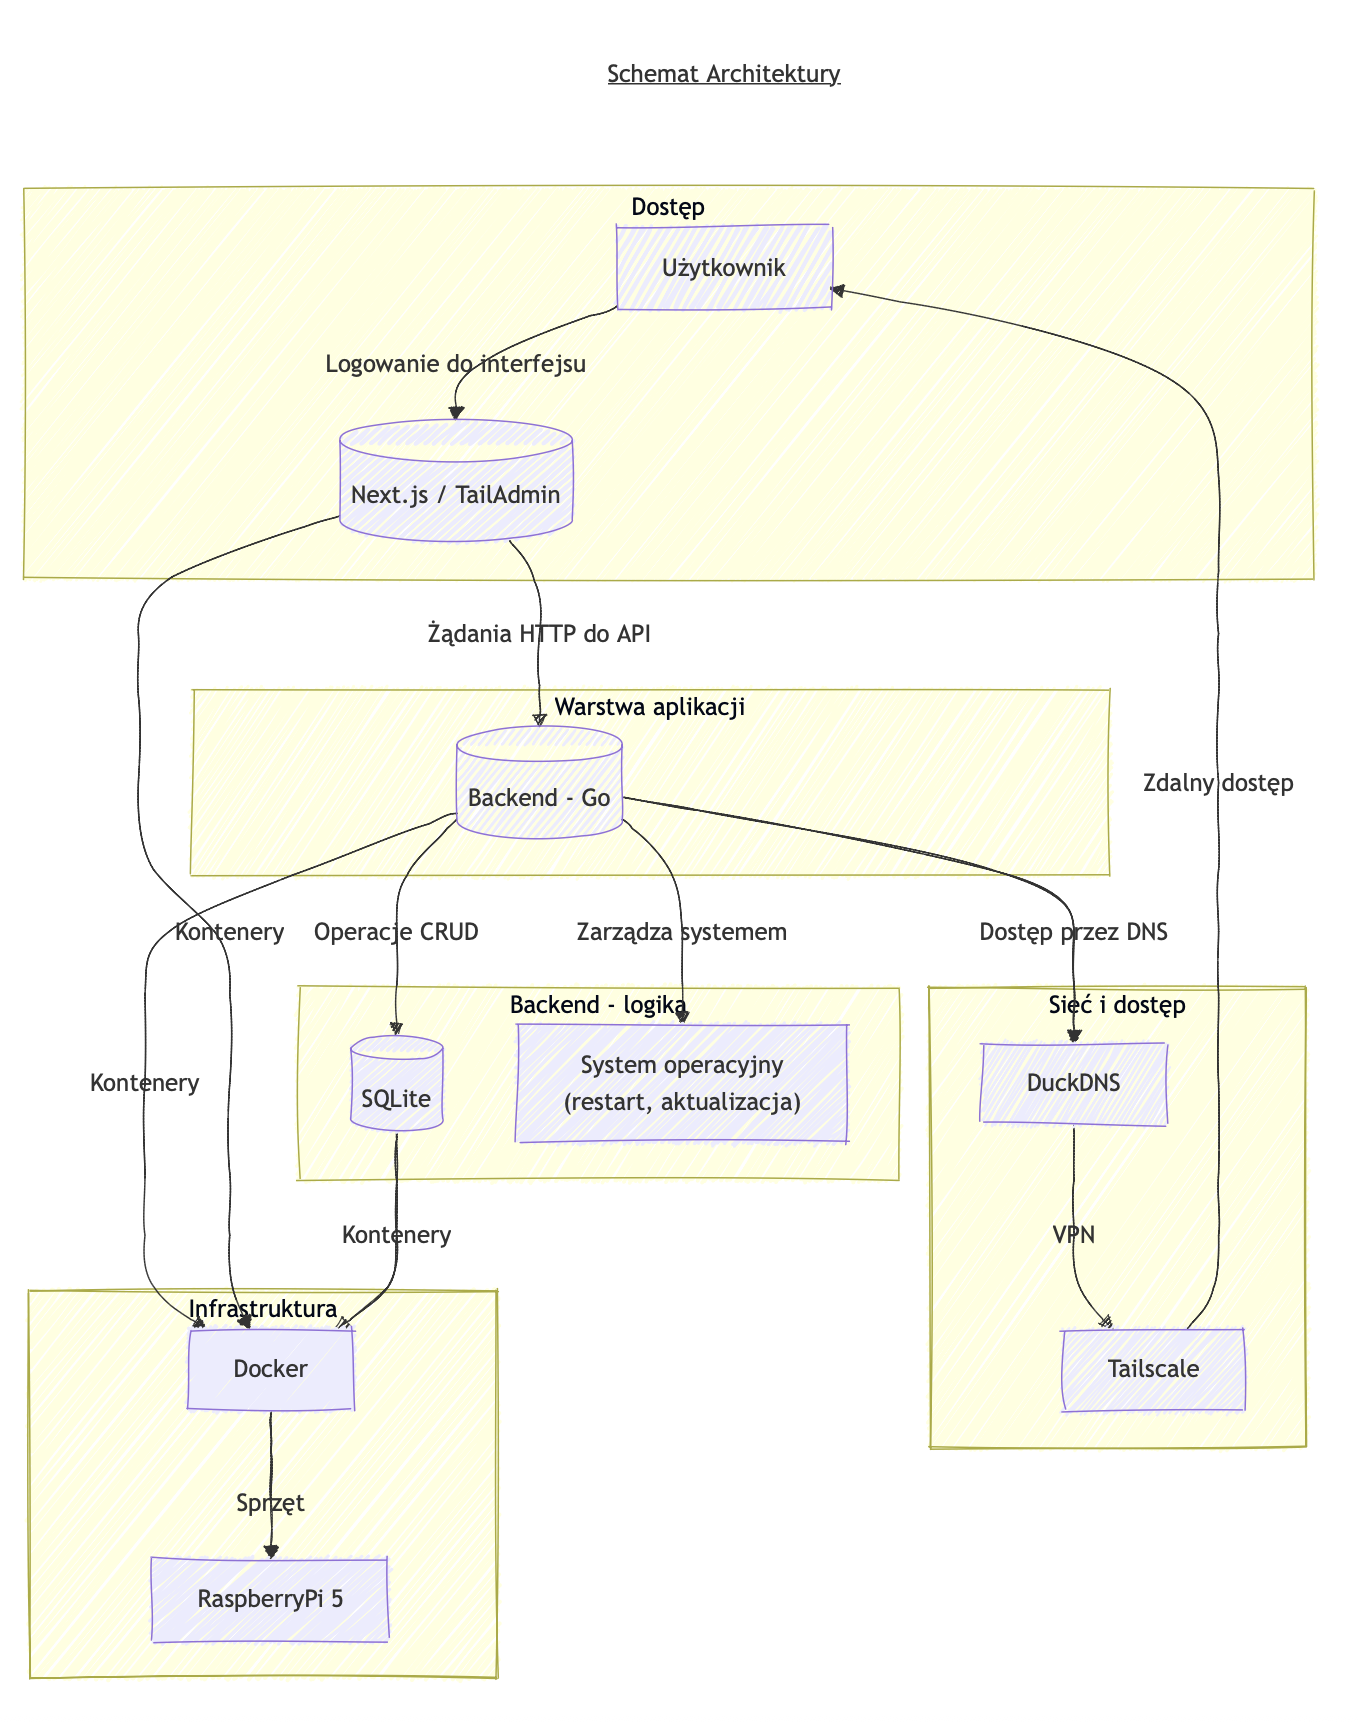
\includegraphics[width=0.8\textwidth]{./chapters/mermeid/schemat_architektury_updated.png}
    \caption{Schemat architektury działania i komunikacji wewnątrz stworzonego systemu.}
    \label{fig:architecture_app}
  \end{figure}
Rysunek 3.1 przedstawia ogólną architekturę systemu HomeLab, ukazującą zależności pomiędzy jego głównymi komponentami. Użytkownik uzyskuje dostęp do systemu poprzez interfejs oparty na Next.js i TailAdmin. Interfejs ten komunikuje się z backendem napisanym w języku Go, który realizuje logikę biznesową oraz zarządza systemem operacyjnym i kontenerami Docker. Dane konfiguracyjne przechowywane są w bazie SQLite. System umożliwia zdalny dostęp dzięki integracji z Tailscale (VPN) oraz DuckDNS (dynamiczny DNS). Całość uruchamiana jest na platformie Raspberry Pi 5, co zapewnia niskie zużycie energii i niski koszt utrzymania.
\subsection{Diagram przepływu danych}
W celu lepszego zrozumienia interakcji pomiędzy komponentami systemu, poniżej przedstawiono diagram przepływu danych ilustrujący komunikację pomiędzy frontendem, backendem, bazą danych oraz zewnętrznymi usługami:
\begin{figure}[H]
    \centering
    \includegraphics[width=0.9\textwidth]{./chapters/mermeid/schemat przepływ danych.png}
    \caption{Diagram przepływu danych w systemie HomeLab.}
    \label{fig:data_flow}
\end{figure}

Rysunek 3.2 przedstawia przepływ danych oraz interakcje pomiędzy głównymi komponentami systemu HomeLab. Użytkownik komunikuje się z interfejsem frontendowym (TailAdmin), który z kolei wykonuje żądania HTTP do API opartego na backendzie napisanym w Go z wykorzystaniem frameworka Gin. Backend odpowiada za obsługę logiki biznesowej, zarządzanie kontenerami Docker, wykonywanie operacji na bazie danych SQLite oraz odczyt parametrów systemu operacyjnego. Informacje o stanie systemu są pobierane przy użyciu narzędzi CLI, takich jak \texttt{df}, \texttt{free}, \texttt{top} oraz \texttt{speedtest}, a następnie zapisywane w bazie danych lub zwracane do interfejsu użytkownika.

\subsection{Backend (Go + SQLite)}
\begin{itemize}
    \item Backend został w całości zaimplementowany w języku Go. Odpowiada za całą logikę biznesową aplikacji oraz komunikację z systemem operacyjnym i środowiskiem kontenerowym Docker.
    \item Aplikacja backendowa zarządza stanem usług, umożliwia ich uruchamianie, zatrzymywanie oraz monitorowanie.
    \item Dane systemowe oraz informacje o użytkownikach przechowywane są lokalnie w lekkiej bazie danych SQLite, co eliminuje konieczność stosowania zewnętrznego serwera baz danych i upraszcza wdrożenie.
    \item Backend może być uruchamiany zarówno jako kontener Docker, jak i jako lokalna aplikacja zainstalowana bezpośrednio na systemie operacyjnym.
\end{itemize}

\textbf{Przykładowy fragment kodu CLI w Go odpowiedzialny za start kontenera:}
\begin{lstlisting}
package main

import (
    "fmt"
    "os/exec"
)

func startContainer(containerName string) error {
    cmd := exec.Command("docker", "start", containerName)
    output, err := cmd.CombinedOutput()
    if err != nil {
        return fmt.Errorf("failed to start container: %s, %v", output, err)
    }
    fmt.Printf("Container %s started successfully\n", containerName)
    return nil
}

func main() {
    if err := startContainer("homelab_service"); err != nil {
        fmt.Println(err)
    }
}
\end{lstlisting}

\subsection{Frontend (TailAdmin)}
\begin{itemize}
    \item Interfejs użytkownika oparty został o szablon TailAdmin, wykorzystujący technologię Next.js i Tailwind CSS.
    \item Frontend zapewnia nowoczesny, responsywny i intuicyjny interfejs do zarządzania usługami systemu, monitorowania zasobów i konfiguracji ustawień.
    \item Aplikacja frontendowa komunikuje się z backendem za pomocą REST API.
    \item Podobnie jak backend, może być uruchamiana jako kontener lub jako statyczna aplikacja hostowana lokalnie.
\end{itemize}

\textbf{Przykładowy fragment kodu React/JSX używanego do pobrania danych systemowych:}
\begin{lstlisting}
import React, { useEffect, useState } from 'react';

function SystemStatus() {
  const [status, setStatus] = useState(null);

  useEffect(() => {
    fetch('/api/system/status')
      .then(res => res.json())
      .then(data => setStatus(data))
      .catch(err => console.error(err));
  }, []);

  if (!status) return <div>Loading...</div>;

  return (
    <div>
      <h2>Status Systemu</h2>
      <p>CPU: {status.cpuUsage}%</p>
      <p>RAM: {status.memoryUsage} MB</p>
      <p>Dysk: {status.diskSpace} GB wolne</p>
    </div>
  );
}

export default SystemStatus;
\end{lstlisting}

\subsection{Warstwa sieciowa}
\begin{itemize}
    \item Połączenia z systemem realizowane są za pomocą sieci VPN opartej o Tailscale, co zapewnia bezpieczny zdalny dostęp bez konieczności stosowania przekierowań portów i stałych adresów IP.
    \item DuckDNS służy jako system dynamicznego DNS, umożliwiając dostęp do systemu za pomocą przyjaznej domeny.
\end{itemize}
\subsubsection{Topologia sieci HomeLaba}
Aby lepiej zobrazować środowisko, w którym działa system HomeLab, przedstawiono przykładową mapę sieci urządzeń i połączeń w typowej konfiguracji domowej. Schemat ilustruje powiązania między kluczowymi komponentami: serwerem głównym, NAS-em, Raspberry Pi, urządzeniami użytkownika oraz systemami zdalnego dostępu.

\begin{figure}[H]
\centering
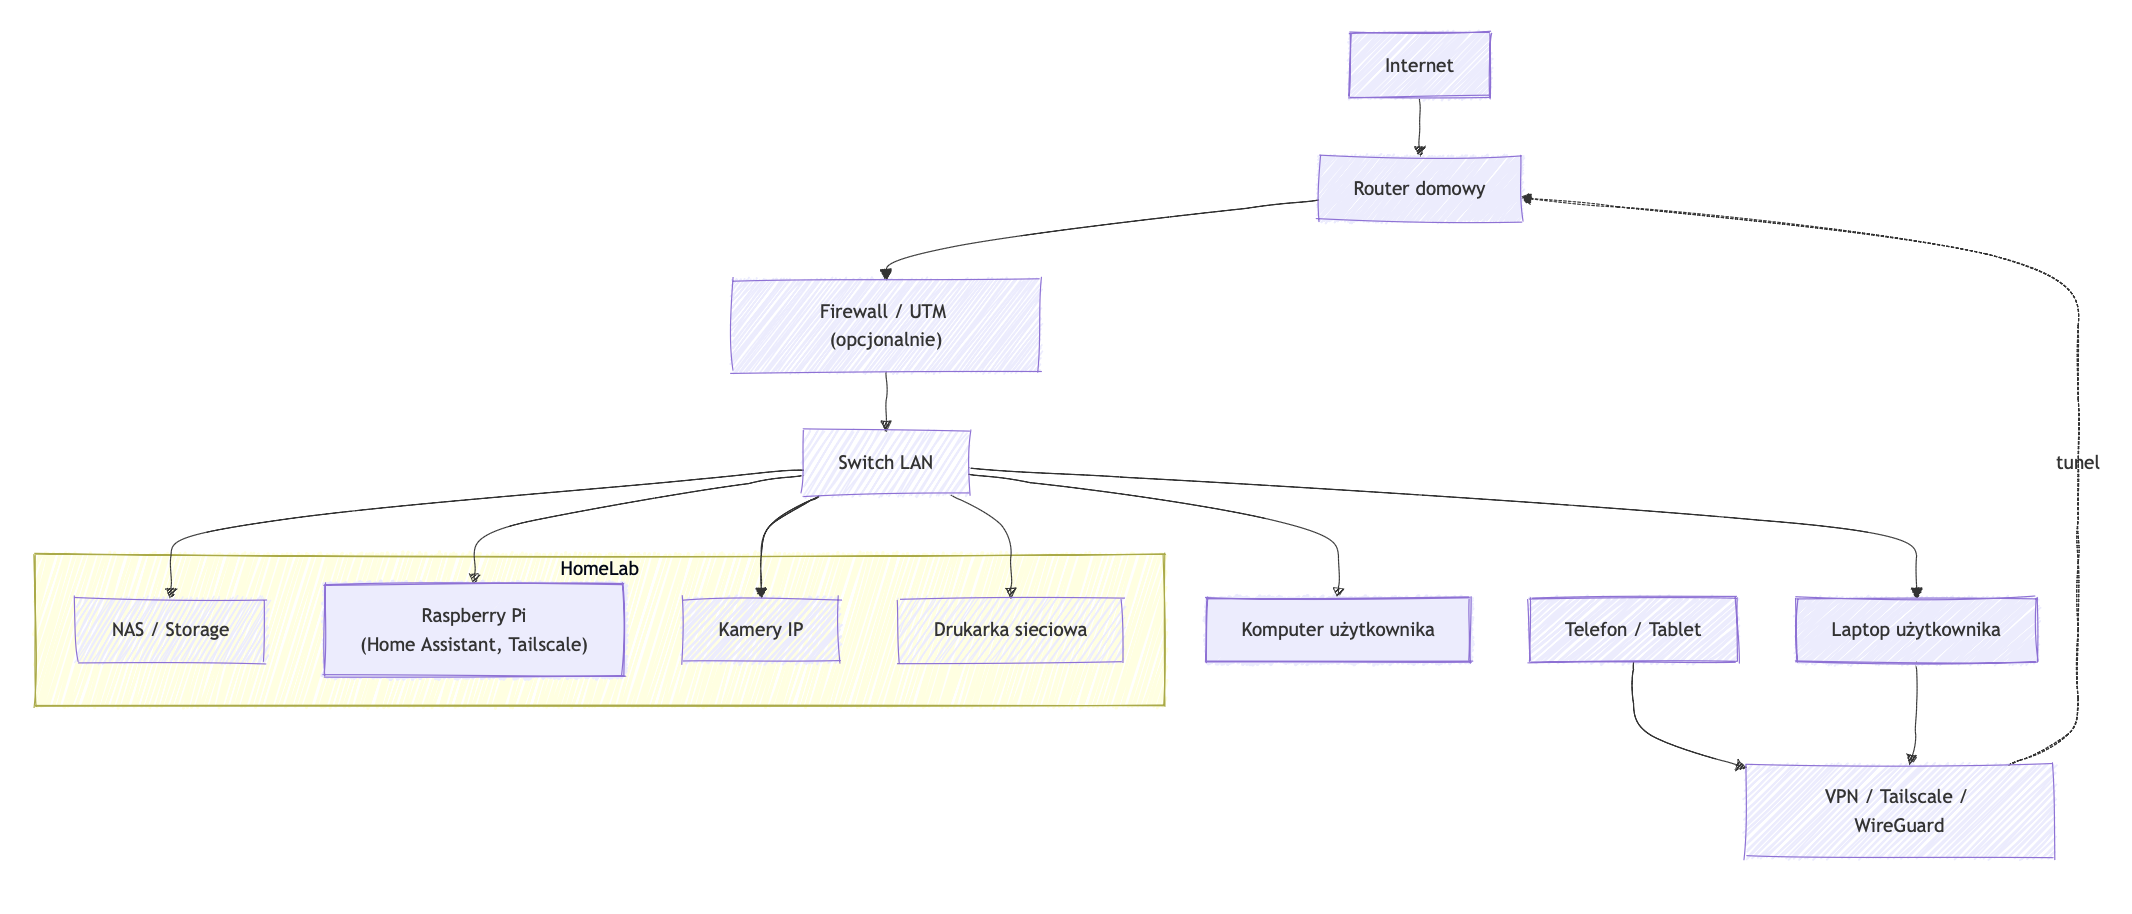
\includegraphics[width=0.95\textwidth]{./chapters/mermeid/schemat sieci homelab.png}
\caption{Mapa sieci HomeLaba z uwzględnieniem kluczowych komponentów i połączeń.}
\label{fig:network_map}
\end{figure}
\textbf{Przykładowa konfiguracja Tailscale z urządzeniem:}

\begin{lstlisting}
# Instalacja Tailscale na Raspberry Pi
curl -fsSL https://tailscale.com/install.sh | sh

# Uruchomienie i logowanie do sieci Tailscale
sudo tailscale up --authkey tskey-xxxxxxxxxxxx

# Sprawdzenie statusu polaczenia
tailscale status
\end{lstlisting}

Konfiguracja umożliwia urządzeniu automatyczne połączenie się z siecią VPN Tailscale, co pozwala na bezpieczny dostęp zdalny do usług HomeLab bez konieczności konfiguracji przekierowań portów.

\subsection{Środowisko kontenerowe}
\begin{itemize}
    \item Docker wykorzystywany jest do zarządzania usługami uruchamianymi w ramach HomeLaba.
    \item System umożliwia instalowanie, uruchamianie i monitorowanie usług jako niezależnych kontenerów, bez potrzeby ręcznej ingerencji użytkownika.
    \item Sam system może być uruchamiany jako kontener lub lokalnie, ale niezależnie od tego zarządza innymi kontenerami poprzez lokalne API Dockera.
\end{itemize}

\subsection{Automatyzacja CI/CD}
\begin{itemize}
    \item GitHub Actions odpowiadają za automatyczne uruchamianie testów jednostkowych oraz analizę statyczną kodu (linter) po każdej zmianie w repozytorium.
    \item Po pomyślnym przejściu testów generowana jest nowa wersja aplikacji backendowej, frontendowej oraz instalatora.
    \item Nowa wersja publikowana jest jako release na GitHubie.
    \item Nie dochodzi do automatycznego wdrożenia na urządzeniu produkcyjnym - użytkownik sam decyduje o pobraniu i uruchomieniu nowej wersji.
\end{itemize}

\textbf{Przykładowy plik `.github/workflows/build.yml`:}
\begin{lstlisting}
name: Build and Test

on:
  push:
    branches:
      - main
  pull_request:

jobs:
  build:
    runs-on: ubuntu-latest

    steps:
    - uses: actions/checkout@v3

    - name: Set up Go
      uses: actions/setup-go@v3
      with:
        go-version: 1.20

    - name: Build Backend
      run: go build -v ./backend/...

    - name: Run Backend Tests
      run: go test -v ./backend/...

    - name: Build Frontend
      run: |
        cd frontend
        npm install
        npm run build

    - name: Run Frontend Tests
      run: |
        cd frontend
        npm test

    - name: Create Release
      uses: softprops/action-gh-release@v1
      with:
        tag_name: ${{ github.ref }}
      env:
        GITHUB_TOKEN: ${{ secrets.GITHUB_TOKEN }}
\end{lstlisting}
\subsection{Wizualizacja procesu CI/CD}
Dla pełnego zrozumienia cyklu automatyzacji wdrożenia systemu, przedstawiono uproszczony wykres przepływu operacji CI/CD:
\begin{figure}[H]
    \centering
    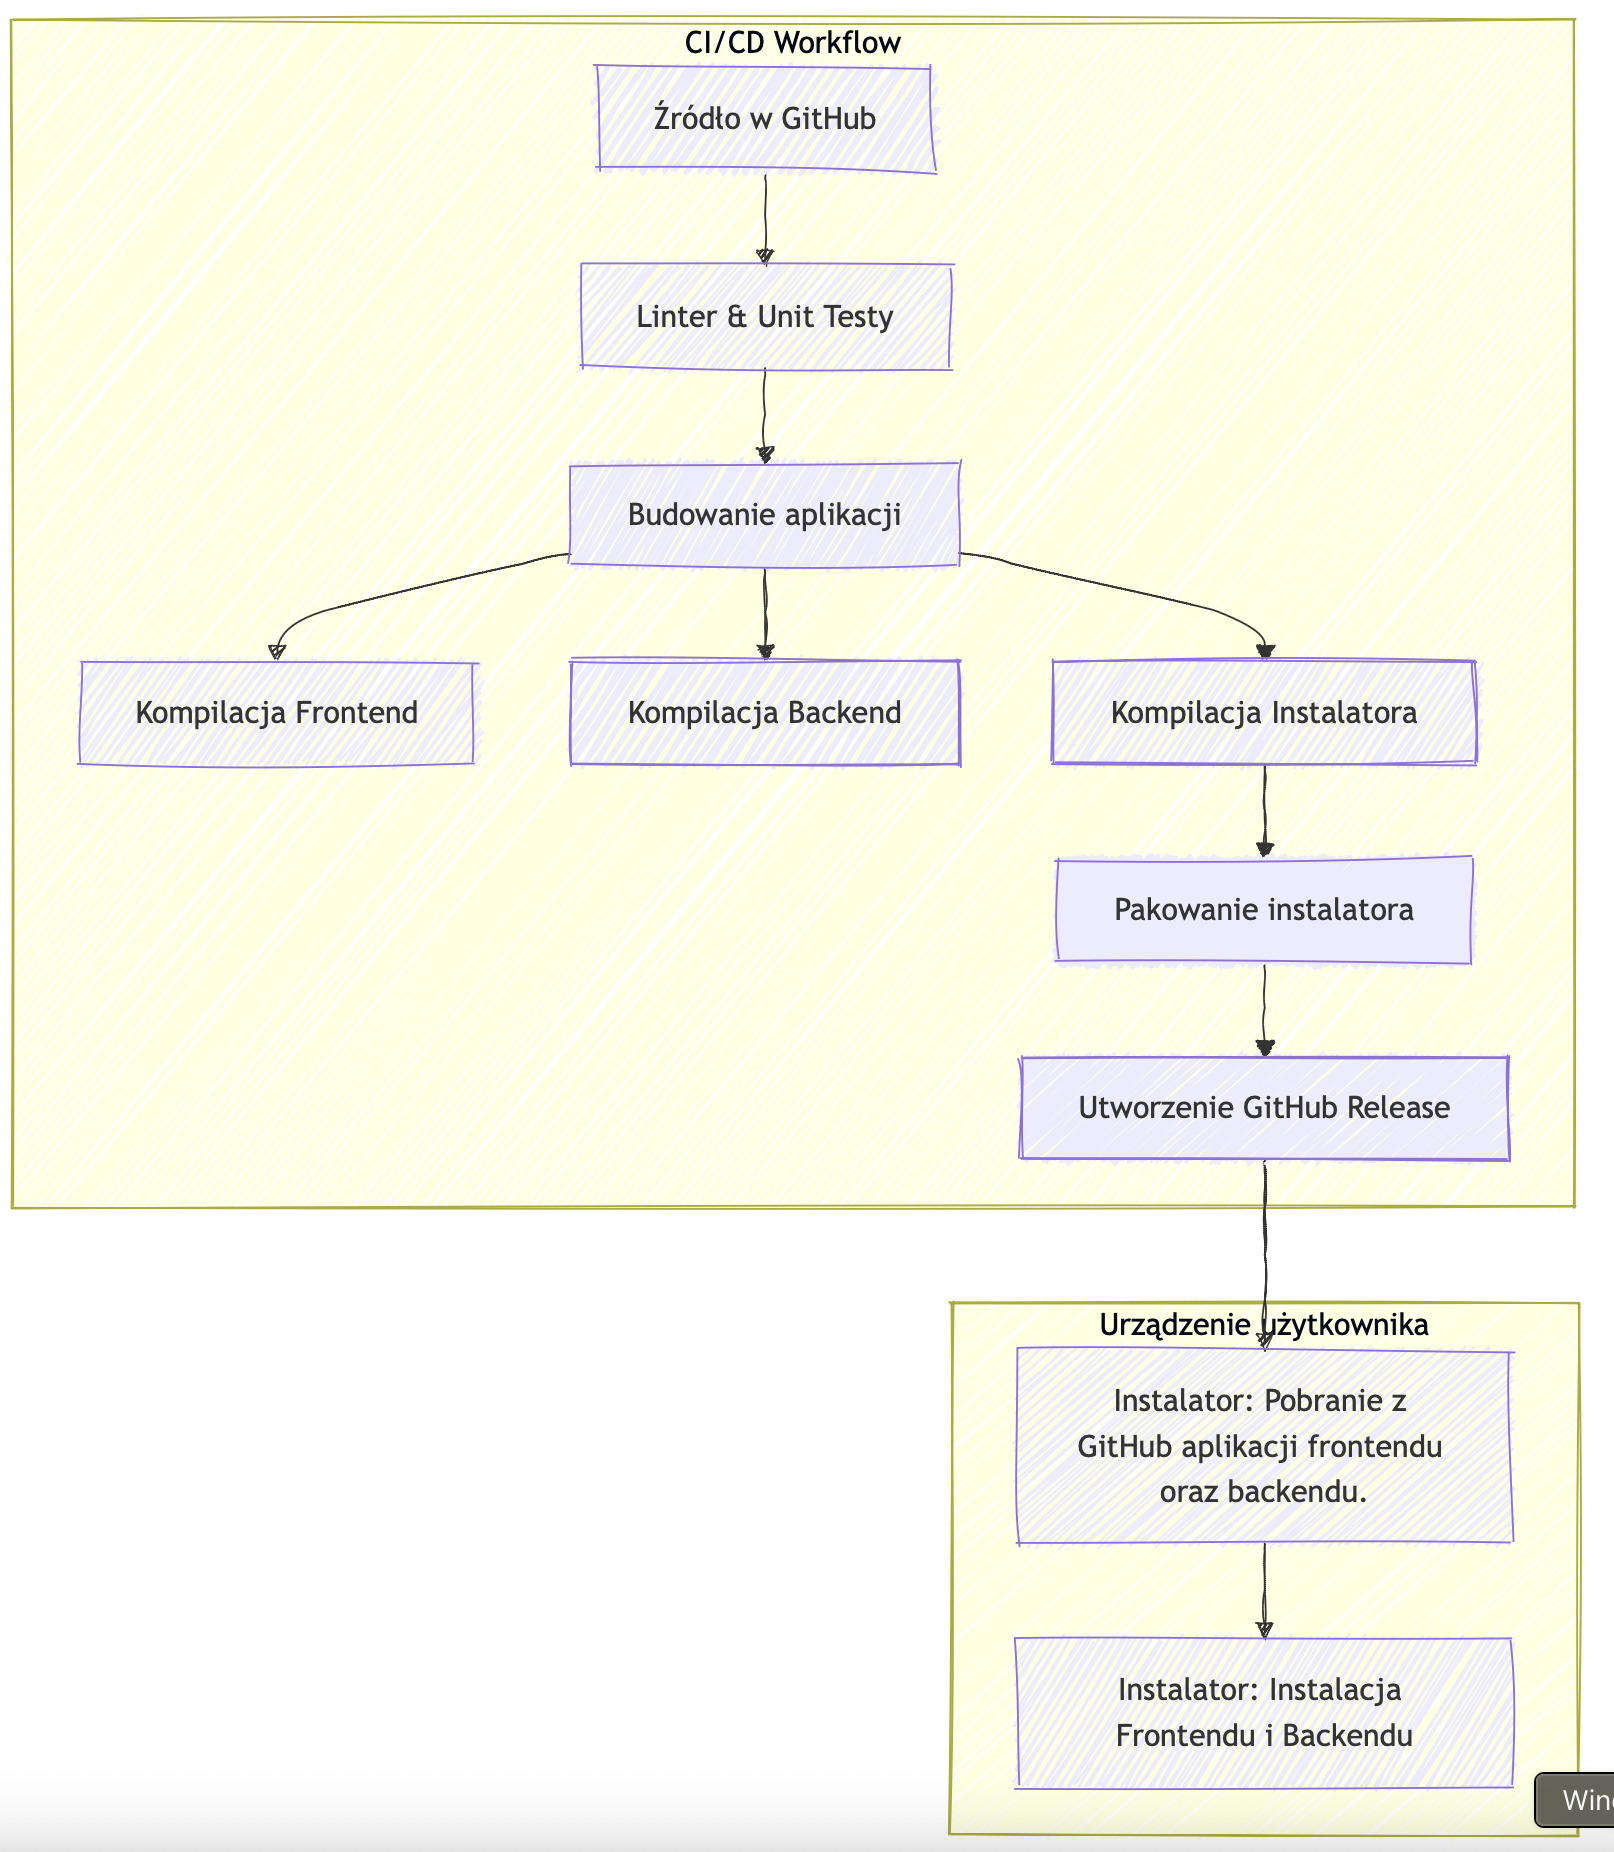
\includegraphics[width=0.90\textwidth]{./chapters/mermeid/schematcicd.png}
    \caption{Schemat procesu CI/CD od momentu zatwierdzenia zmiany aż do utworzenia wydania.}
    \label{fig:ci_cd_pipeline}
\end{figure}

Diagram przedstawia proces automatyzacji CI/CD zastosowany w projekcie HomeLab. Cały proces rozpoczyna się od zatwierdzenia zmian w repozytorium GitHub, co uruchamia mechanizm testów jednostkowych oraz analizę statyczną kodu (linter). Następnie aplikacja jest budowana - zarówno frontend, backend, jak i instalator. Po zakończeniu kompilacji instalator zostaje spakowany, a całość publikowana w formie GitHub Release. Użytkownik końcowy może następnie pobrać instalator, który automatycznie pobierze najnowsze wersje komponentów z GitHuba i zainstaluje je lokalnie.

\subsection{Urządzenie docelowe}

System docelowo uruchamiany jest na urządzeniu Raspberry Pi 5, które zapewnia odpowiednią wydajność przy bardzo niskim zużyciu energii. Dzięki temu możliwe jest ciągłe działanie systemu w warunkach domowych, przy minimalnych kosztach utrzymania.
\section{Technologie i narzędzia uzyte w systemie}

System HomeLab wykorzystuje następujące technologie:
\subsection{Backend}
\begin{itemize}
    \item Go - zapewnia wysoką wydajność i prostotę wdrożenia na systemach typu embedded jak Raspberry Pi.
    \item SQLite - lekka, lokalna baza danych eliminująca potrzebę zewnętrznego serwera, idealna do przechowywania konfiguracji i danych użytkowników.
\end{itemize}
\subsection{Frontend}
\begin{itemize}
    \item TailAdmin - nowoczesny szablon interfejsu użytkownika oparty na Next.js i Tailwind CSS, zapewniający responsywność i łatwość rozbudowy.
    \item REST API - umożliwia komunikację między frontendem a backendem w sposób prosty i efektywny.
\end{itemize}
\subsection{Warstwa Sieciowa}
\begin{itemize}
    \item Tailscale - VPN do bezpiecznego zapewnienia zdalnego dostępu do systemu, bez konieczności posiadania stałego adresu IP.
    \item DuckDNS - dynamiczny system zarządzania domeną umożliwiający łatwy dostęp do systemu.
\end{itemize}
\subsection{Środowisko uruchomieniowe}
\begin{itemize}
    \item Docker - uzywany do konteneryzacji aplikacji i zarządzania zależnościami, umożliwiając izolację i łatwe wdrażanie usług.
    \item Raspberry Pi 5 - host systemu zapewniający energooszczędność i niski koszt.
\end{itemize}
\subsection{Automatyzacja CI/CD}
\begin{itemize}
    \item GitHub Actions - narzędzie do automatyzacji wdrożeń i testowania kodu, umożliwiające szybkie i powtarzalne procesy buildów i testów.
    \item Pipeline CI/CD - automatyczne testowanie, budowanie i wdrażanie aplikacji, zwiększające jakość i niezawodność systemu.
\end{itemize}

Dzięki zastosowaniu powyzszych technologii system Homelab będzie nowoczesnym, skalowalnym i energooszczędnym rozwiązaniem dla uzytkowników domowych.

\chapter{Implementacja systemu}

\section{Backend - API do zarządzania systemem}

\subsection{Struktura API i kluczowe endpointy}
\begin{figure}[H]
  \centering
  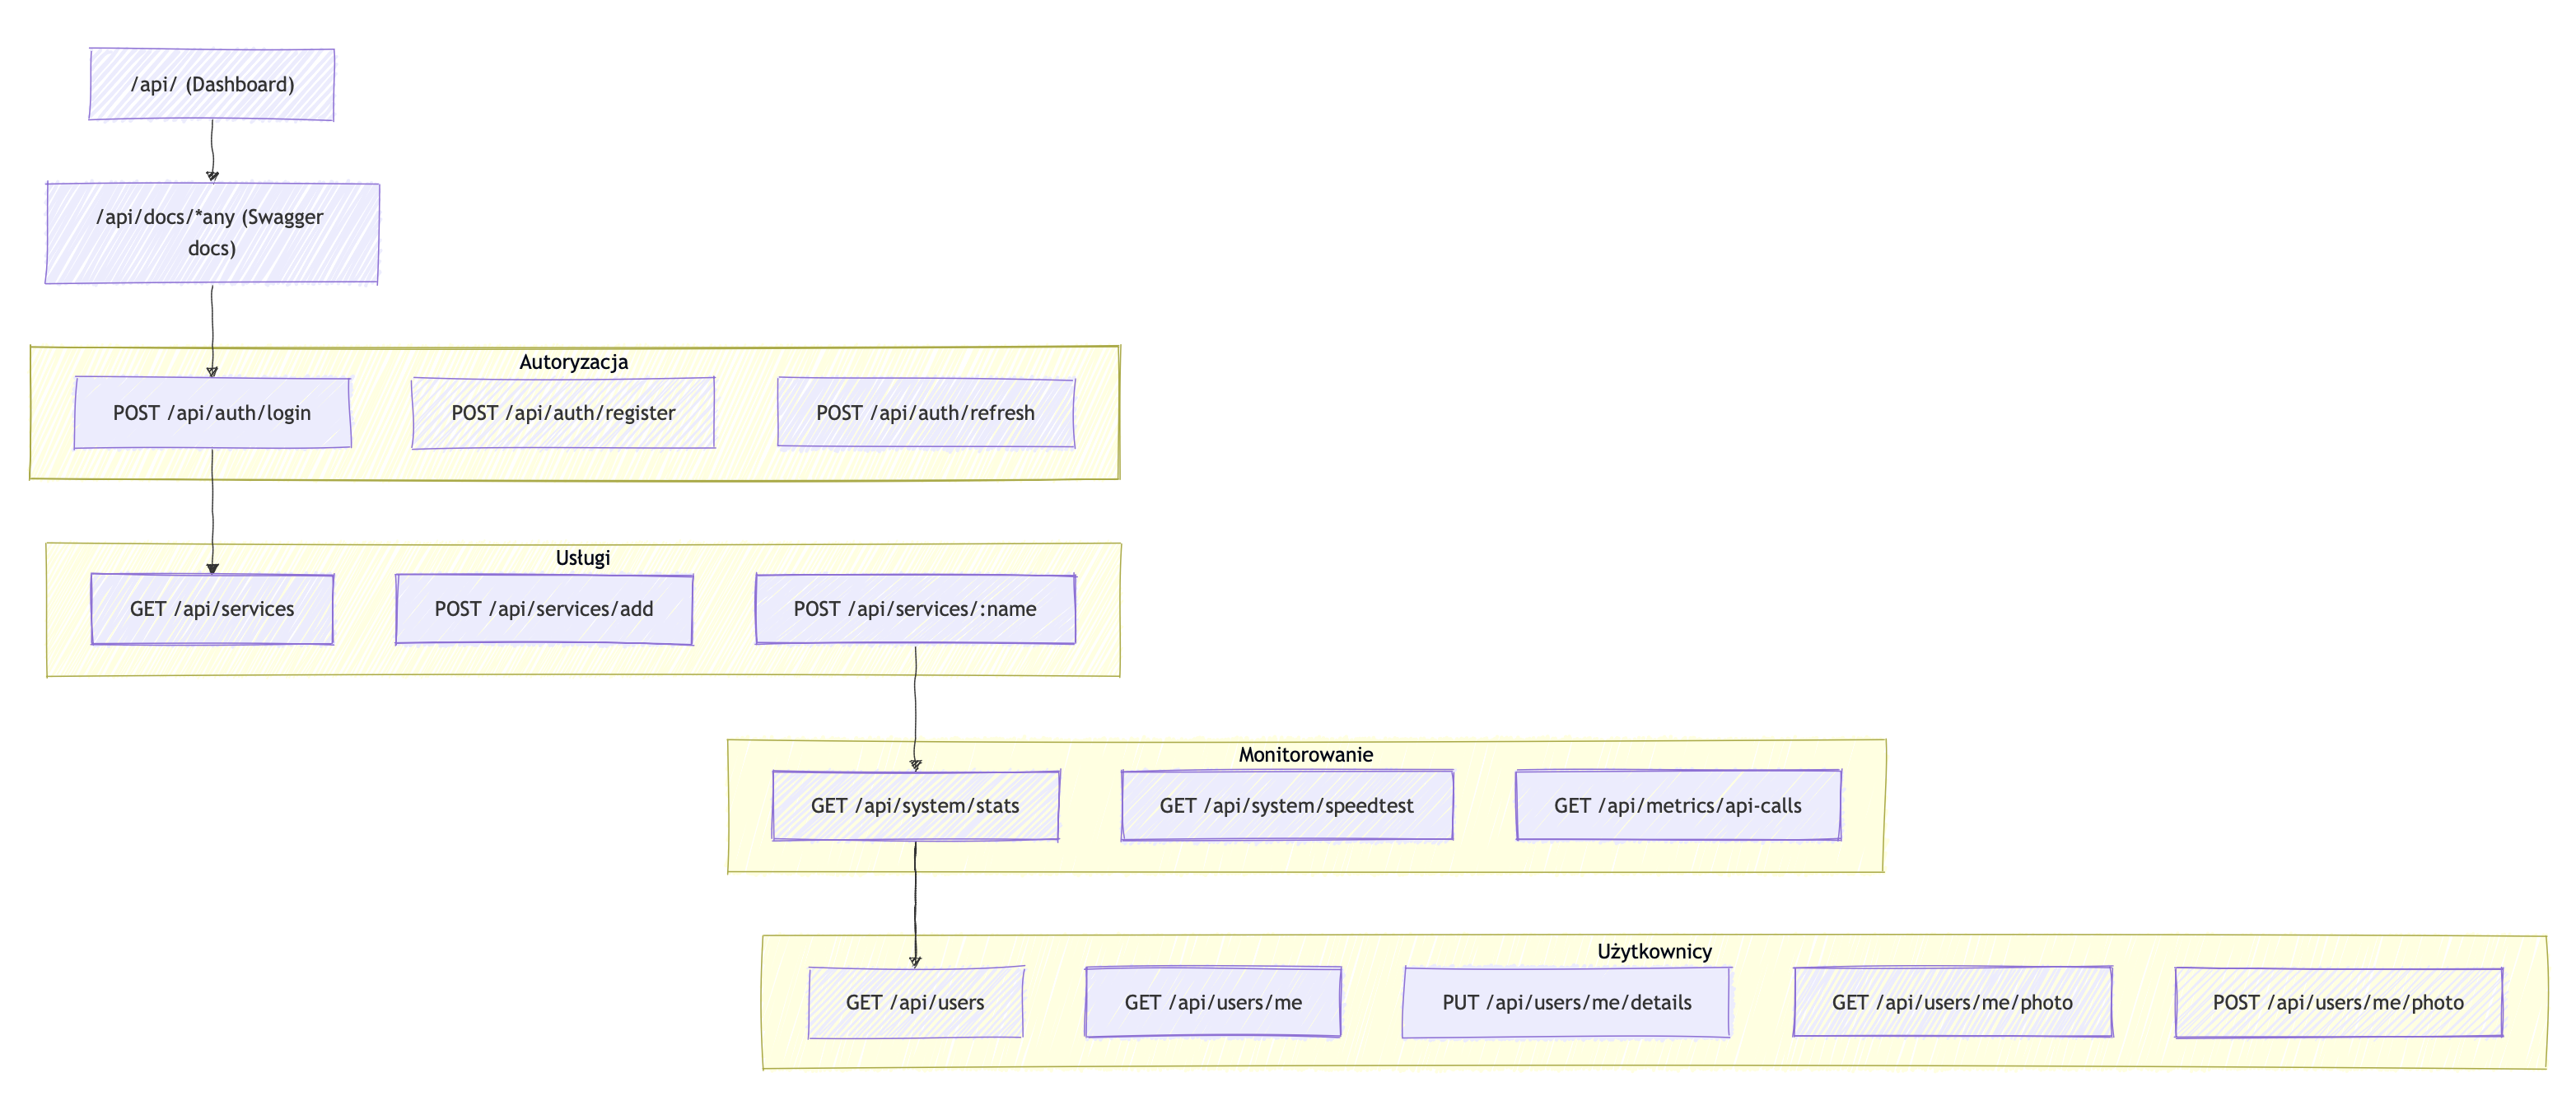
\includegraphics[width=1\textwidth]{./chapters/mermeid/schemat api.png}
  \caption{Schemat architektury API aplikacji HomeNest.}
  \label{fig:api_schema}
\end{figure}
System został zaprojektowany jako aplikacja webowa z backendem opartym na języku Go, wykorzystującym framework Gin, zapewniającym wysoką wydajność oraz możliwość łatwego definiowania tras i obsługi żądań HTTP. API udostępnia szereg endpointów pozwalających na zarządzanie użytkownikami, usługami, monitorowanie systemu oraz uwierzytelnianie.

\subsubsection{Autoryzacja i uwierzytelnianie}
\begin{itemize}
    \item \textbf{POST /api/auth/login} - logowanie użytkownika i zwrócenie tokena JWT,
    \item \textbf{POST /api/auth/register} - rejestracja nowego użytkownika,
    \item \textbf{POST /api/auth/refresh} - odświeżenie tokena JWT.
\end{itemize}

\subsubsection{Zarządzanie usługami}
\begin{itemize}
    \item \textbf{GET /api/services} - pobranie listy aktualnie zarejestrowanych usług,
    \item \textbf{POST /api/services/add} - dodanie nowej usługi do systemu,
    \item \textbf{POST /api/services/:name} - przełączenie (uruchomienie/zatrzymanie) wybranej usługi według nazwy.
\end{itemize}

\subsubsection{Monitorowanie systemu}
\begin{itemize}
    \item \textbf{GET /api/system/stats} - pobranie statystyk systemowych, takich jak zużycie CPU, RAM, przestrzeń dyskowa,
    \item \textbf{GET /api/system/speedtest} - pobranie wyników testu prędkości połączenia internetowego,
    \item \textbf{GET /api/metrics/api-calls} - pobranie liczby zapytań API z ostatnich dni.
\end{itemize}

\subsubsection{Zarządzanie użytkownikami}
\begin{itemize}
    \item \textbf{GET /api/users} - lista użytkowników (dostępna tylko dla administratora),
    \item \textbf{GET /api/users/me} - pobranie danych zalogowanego użytkownika,
    \item \textbf{PUT /api/users/me/details} - aktualizacja danych zalogowanego użytkownika,
    \item \textbf{POST /api/users/me/photo} - przesłanie zdjęcia profilowego,
    \item \textbf{GET /api/users/me/photo} - pobranie zdjęcia profilowego użytkownika.
\end{itemize}

\subsubsection{Dashboard i dokumentacja}
\begin{itemize}
    \item \textbf{GET /api/} - główny endpoint dashboardu aplikacji,
    \item \textbf{GET /api/docs/*any} - dokumentacja API generowana automatycznie przy użyciu narzędzia Swagger.
\end{itemize}

\subsubsection{Podsumowanie}
Zaprojektowane API jest modularne, bezpieczne i łatwe do rozszerzenia. Struktura endpointów została opracowana w sposób zgodny z dobrymi praktykami REST, umożliwiając wygodne zarządzanie zasobami systemowymi i użytkownikami, a dzięki wykorzystaniu frameworka Gin osiągnięto wysoką wydajność obsługi żądań. Endpointy są chronione przez mechanizmy JWT i w zależności od kontekstu użytkownika odpowiednio ograniczają dostęp do operacji administracyjnych.


\subsection{Obsługa uwierzytelniania i autoryzacji}

System uwierzytelniania i autoryzacji opiera się na tokenach JWT (JSON Web Token). Mechanizm ten zapewnia bezpieczną kontrolę dostępu do zasobów systemu, umożliwiając przypisanie użytkownikom odpowiednich ról i ograniczenie dostępu do krytycznych operacji administracyjnych.

\subsubsection{Proces uwierzytelniania}
Każdy użytkownik musi zalogować się do systemu, podając swoje dane uwierzytelniające. Po pomyślnej weryfikacji hasła system generuje token JWT, który służy do autoryzacji kolejnych żądań API. Token zawiera informacje o użytkowniku oraz jego roli w systemie.

Kluczowe endpointy:
\begin{itemize}
    \item \textbf{POST /api/register} – Rejestracja nowego użytkownika,
    \item \textbf{POST /api/login} – Logowanie użytkownika i zwrócenie tokena JWT.
\end{itemize}
\newpage
\section{Frontend - Interfejs uzytkownika}

\subsection{Projekt UI/UX}

Z założenia interfejs użytkownika powinien być jak najprostszy oraz jak najbardziej ułatwiać użytkownikowi korzystanie z systemu. Powininen on umożliwiać użytkownikowi korzystanie z systemu w sposób zamierzony oraz uniemożliwiać korzystanie z systemu w sposób niezgodny z przeznaczeniem.
\subsubsection{Założenia projektowe}
Podstawowe cele projektowe interfejsu obejmowały:
\begin{itemize}
    \item Czytelność i prostota obsługi,
    \item Spójność wizualną oraz intuicyjna nawigacja,
    \item Minimalizacja liczby kliknięć wymaganych do wykonania operacji,
    \item Odpowiednia organizacja informacji w oparciu o hierarchię wizualną.
\end{itemize}

\subsubsection{Struktura interfejsu}
Projekt składa się z kilku widoków które zostaną opisane poniżej:
\paragraph{Strona Główna} - Strona przedstawia statystyki wykorzystania systemu oraz podstawowe informacje dotyczące środowiska uruchomieniowego.
\begin{figure}[H]
  \centering
  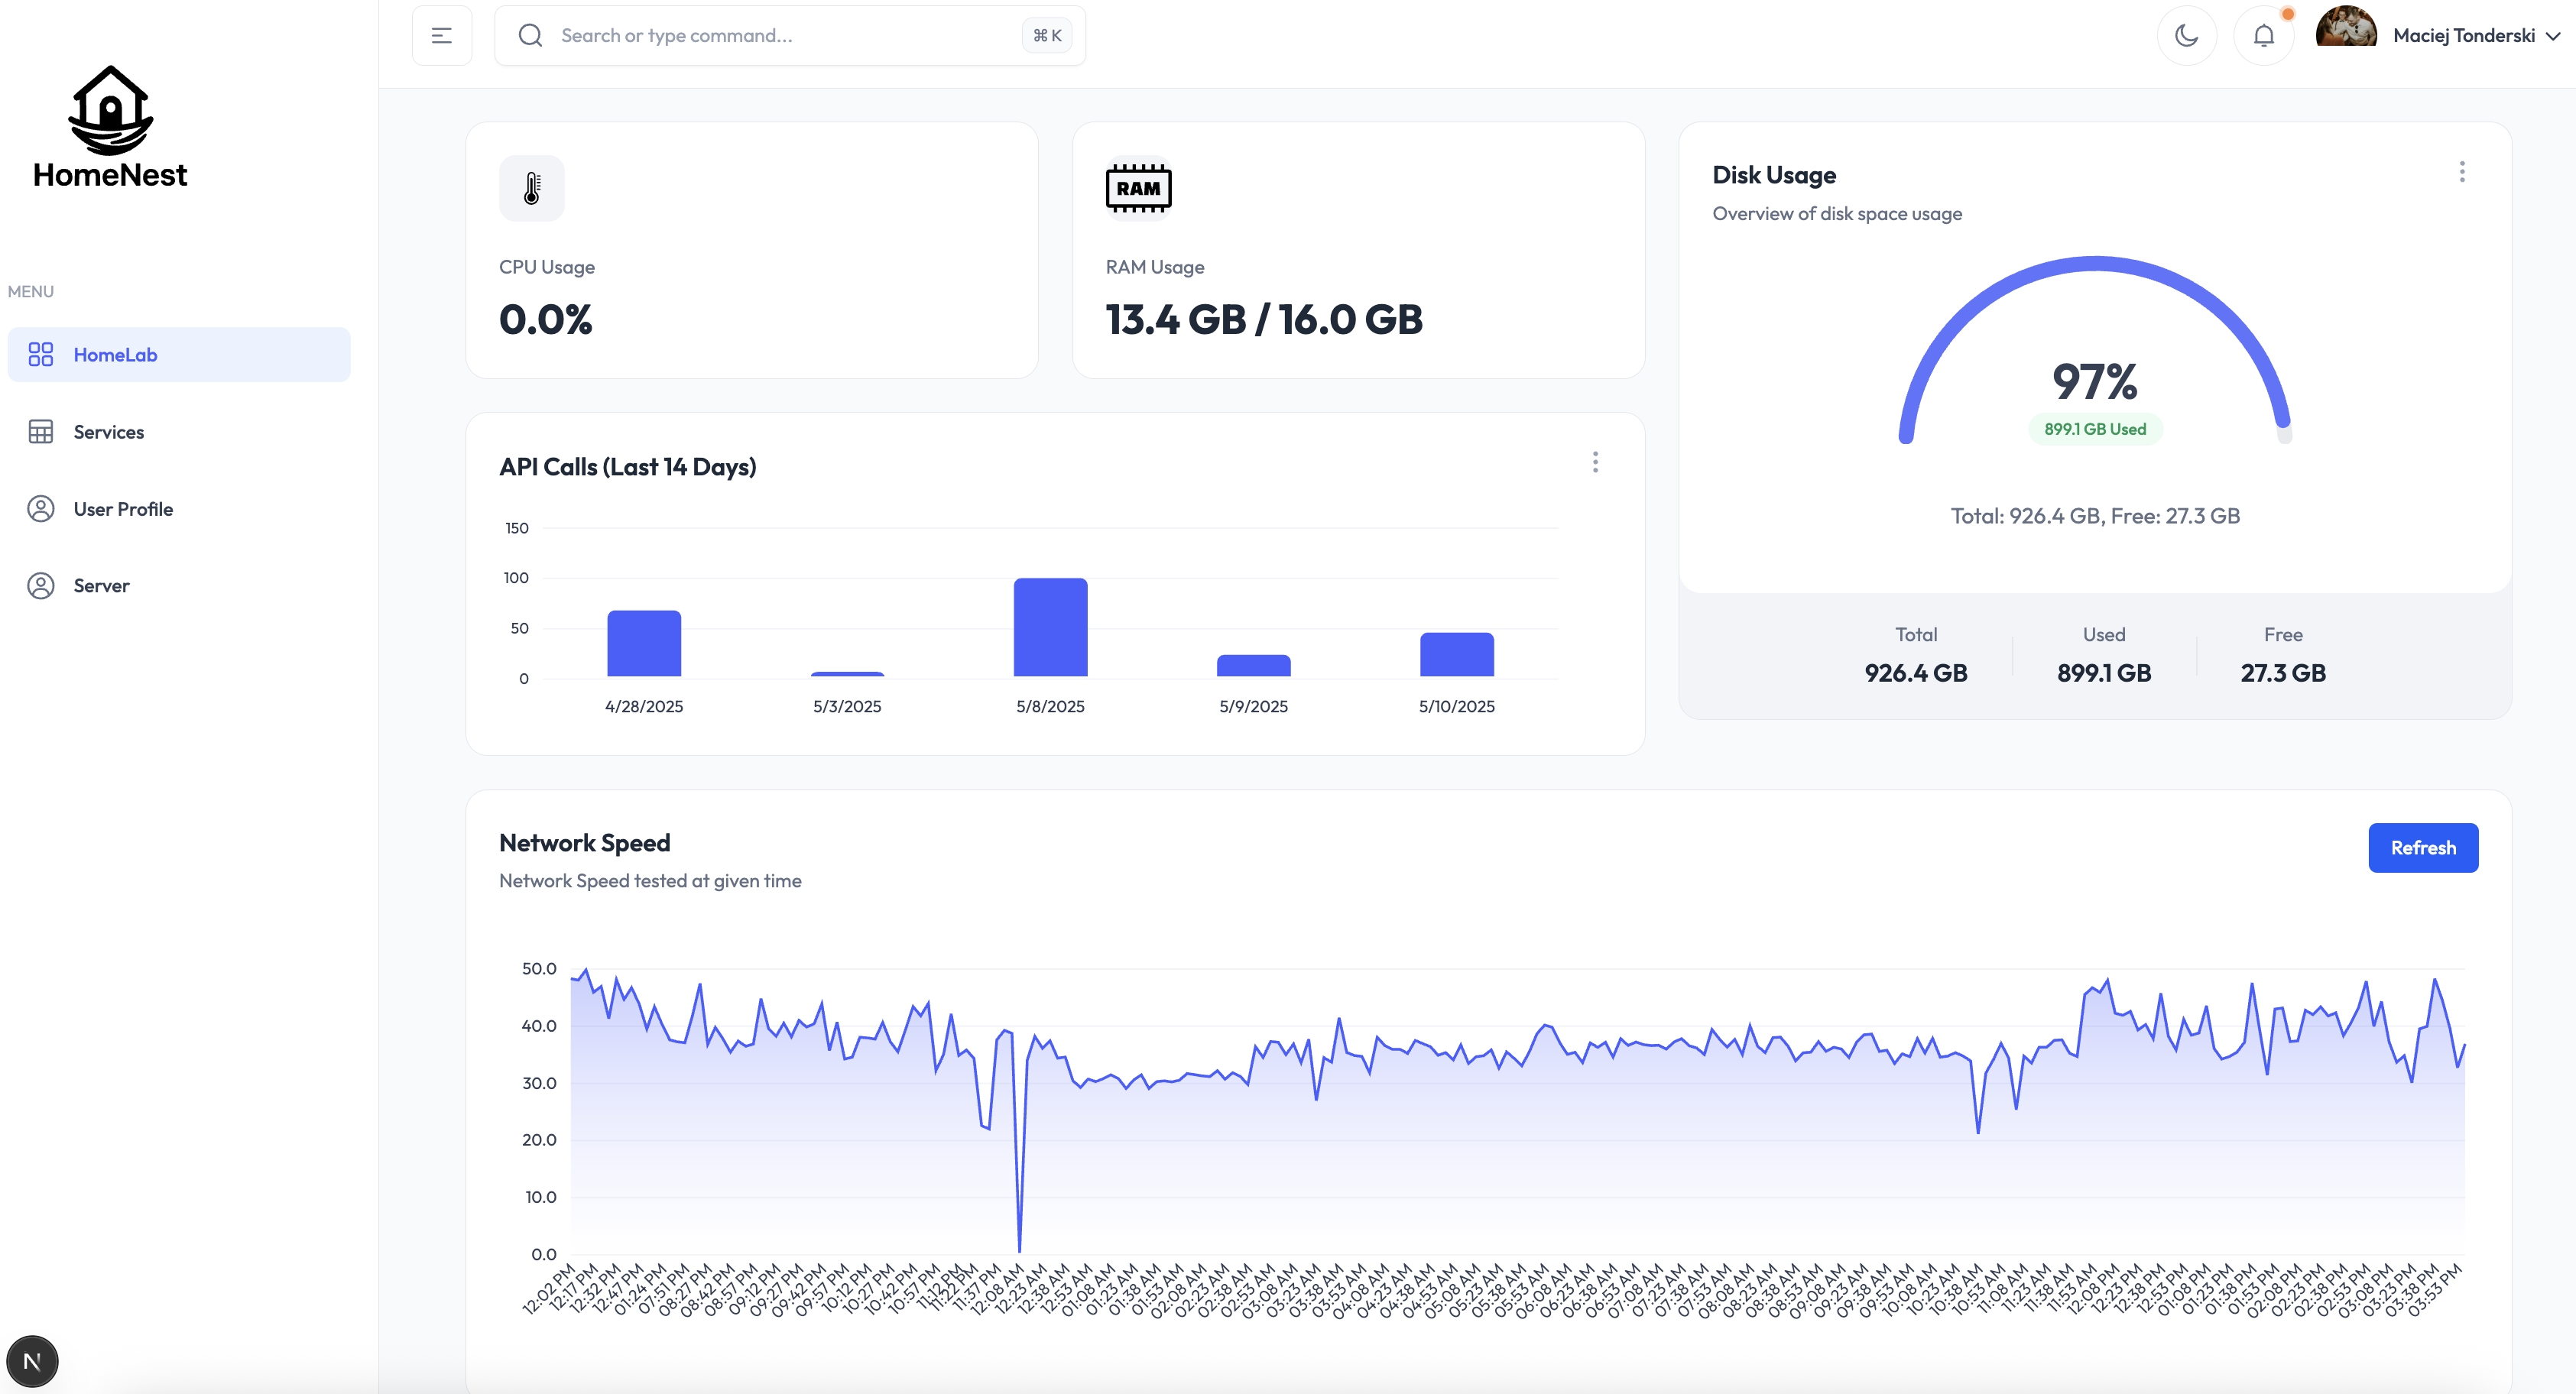
\includegraphics[width=1\textwidth]{./chapters/assets/UI_HomePage.png}
  \caption{Strona główna aplikacji Homelab.}
  \label{fig:ui_homepage}
\end{figure}
\begin{itemize}
    \item \textbf{Panel Informacyjny - wykorzystanie CPU} - Zawiera procentową wartość użycia procesora.
    \item \textbf{Panel Informacyjny - wykorzystanie RAM} - Zawiera informację ile GB pamięci RAM jest obecnie w użyciu oraz dostępną ilość pamięci RAM.
    \item \textbf{Wykres - Wykorzystanie Dysku} - Zawiera informację o wykorzystaniu dysku - ilość zajętej oraz dostępnej przestrzeni dyskowej.
    \item \textbf{Wykres - Ilość zapytań API apilikacji w ostatnich 14 dniach} - Pokazuje ile zapytań do aplikacji API zostało wykonanych w ostatnich 14 danich. Jeżeli aplikacja nie wykonywała zapytań do bazy przez ostatnie 14 dni codziennie umieszczne jest ostatnie 14 wpisów z bazy danych.
    \item \textbf{Wykres - Prędkość internetu} - System zgodnie z harmonogramem sprawdza prędkość podłączonego łącza internetowego i wyświetla je w formie tabeli w tym miejscu.
\end{itemize}

\paragraph{Strona Logowania oraz Rejestracji} - Strona umożliwa użytkownikowi wprowadzenie danych niezbęnych do umożliwienia korzystania z systemu. Użytkownik może się zalogować lub zarejestrować.
\begin{figure}[H]
  \centering
  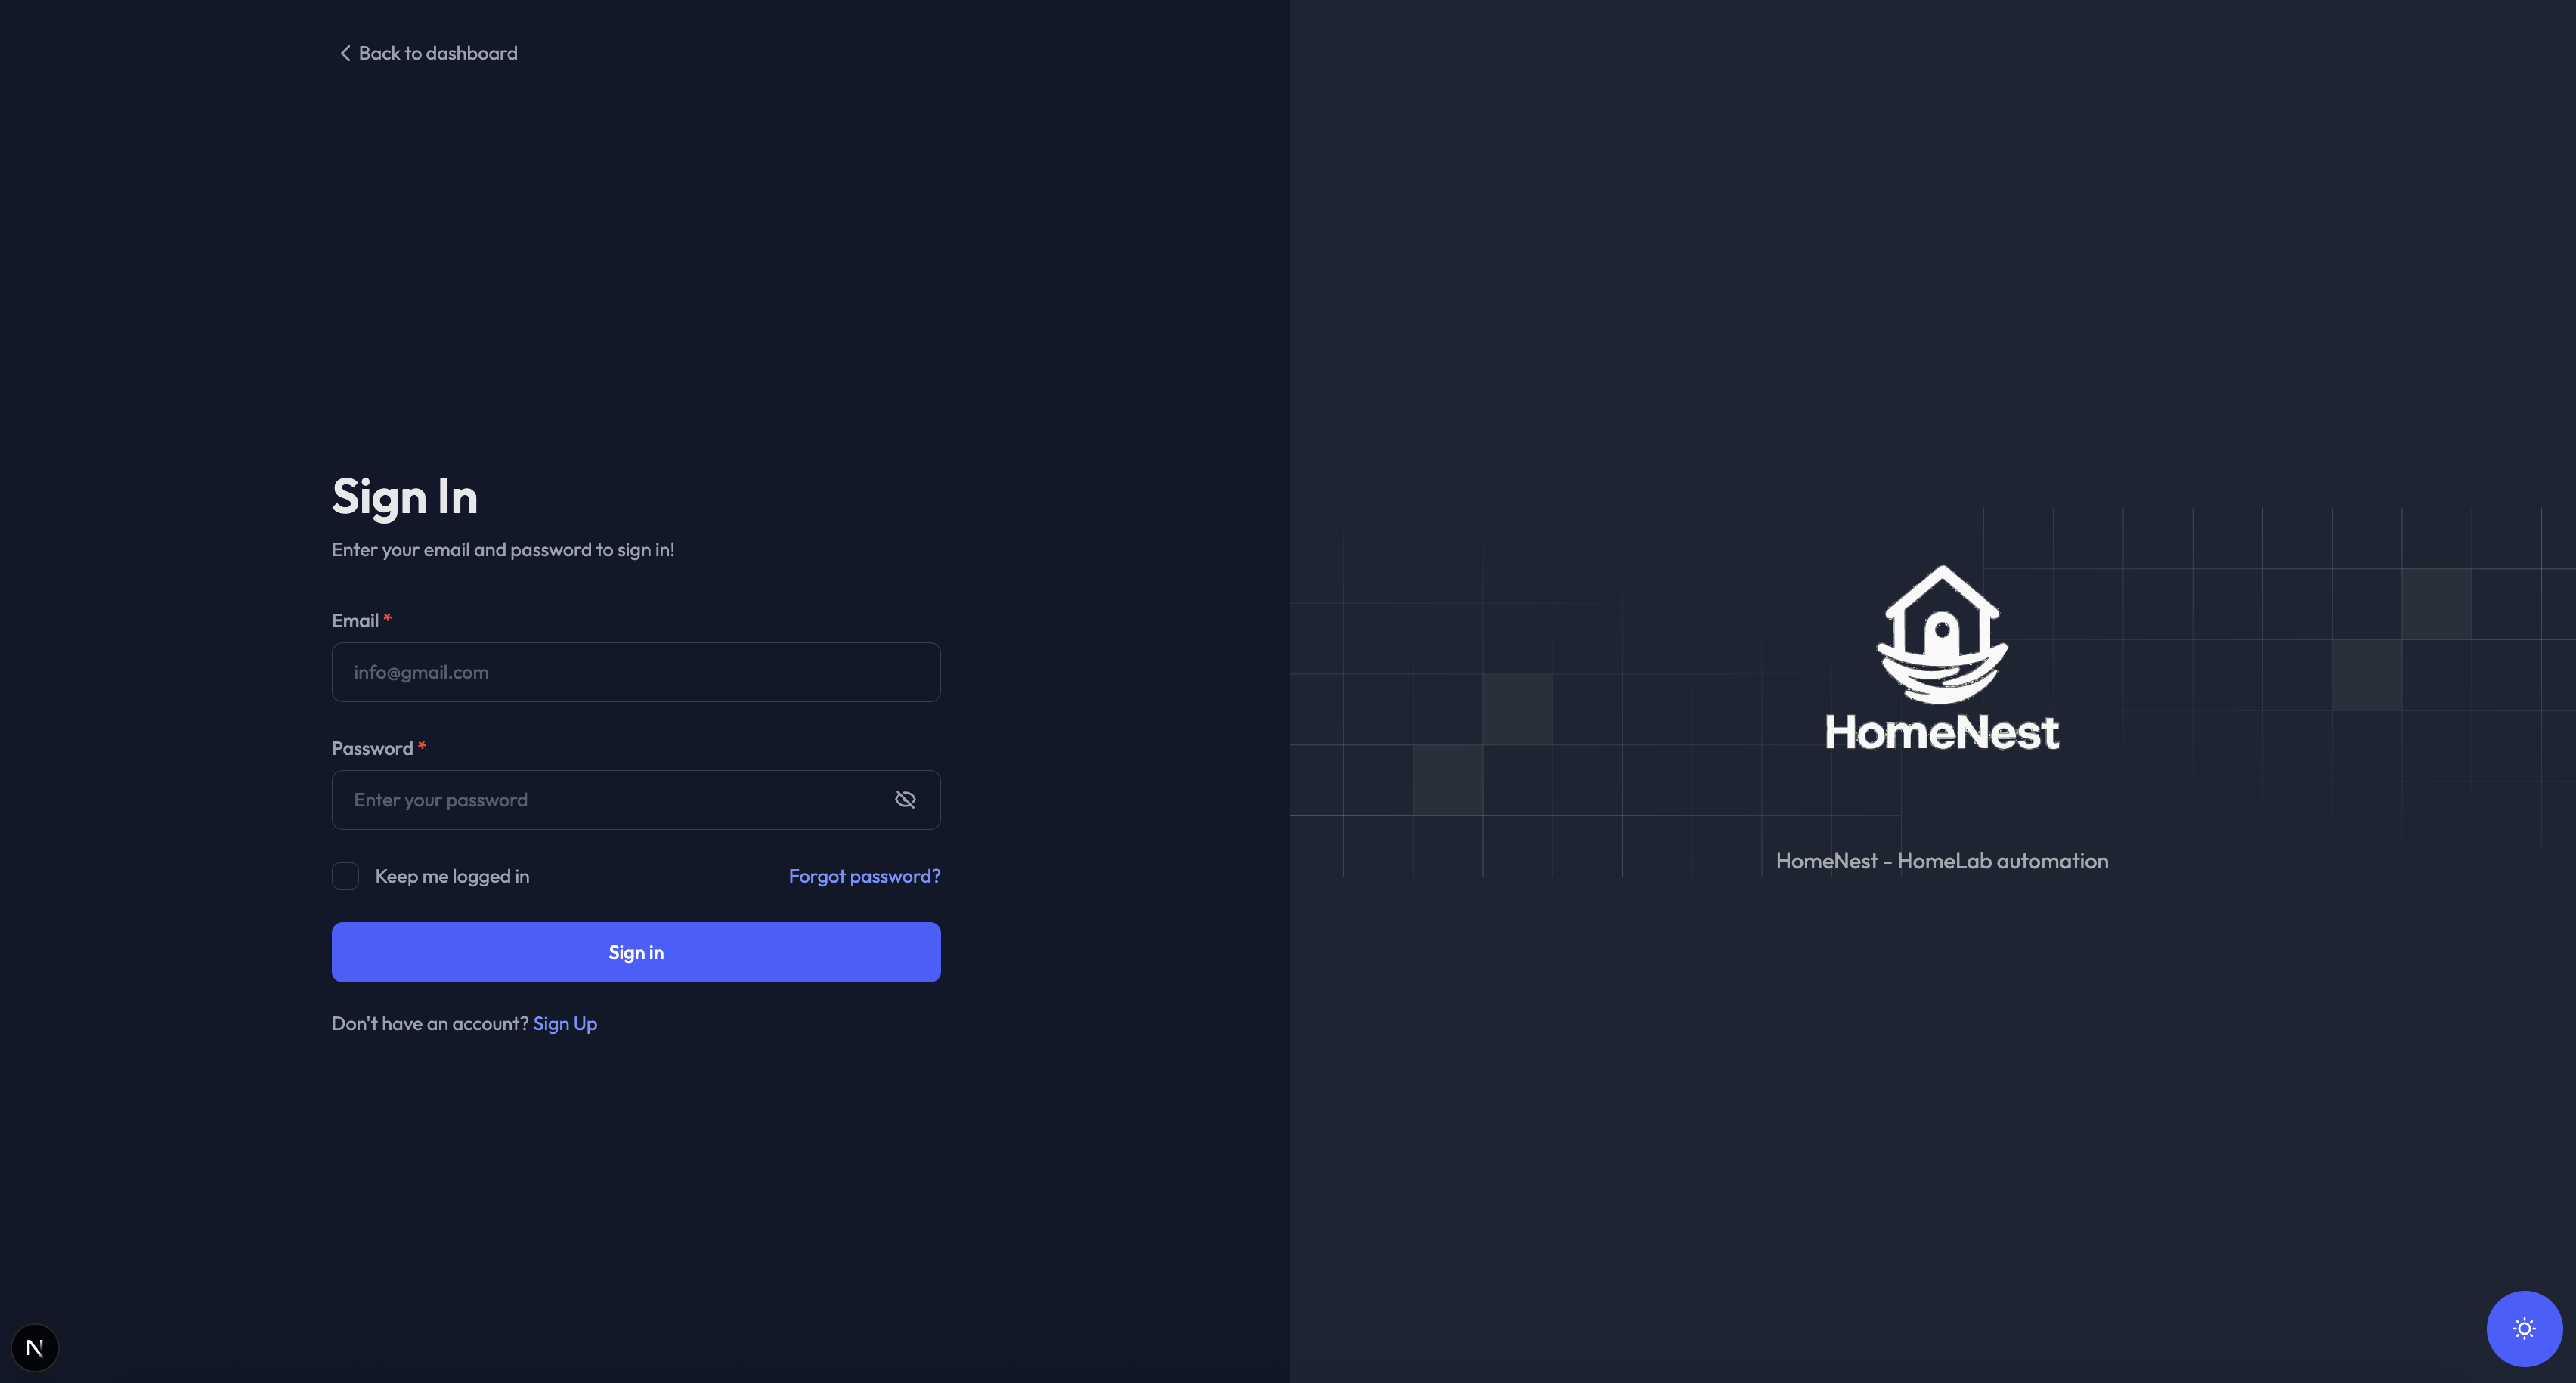
\includegraphics[width=1\textwidth]{./chapters/assets/login_page.png}
  \caption{Strona logowania do serwisu wyświetlająca logo oraz pola do wprowadzenia danych logowania}
  \label{fig:ui_login}
\end{figure}

\begin{figure}[H]
  \centering
  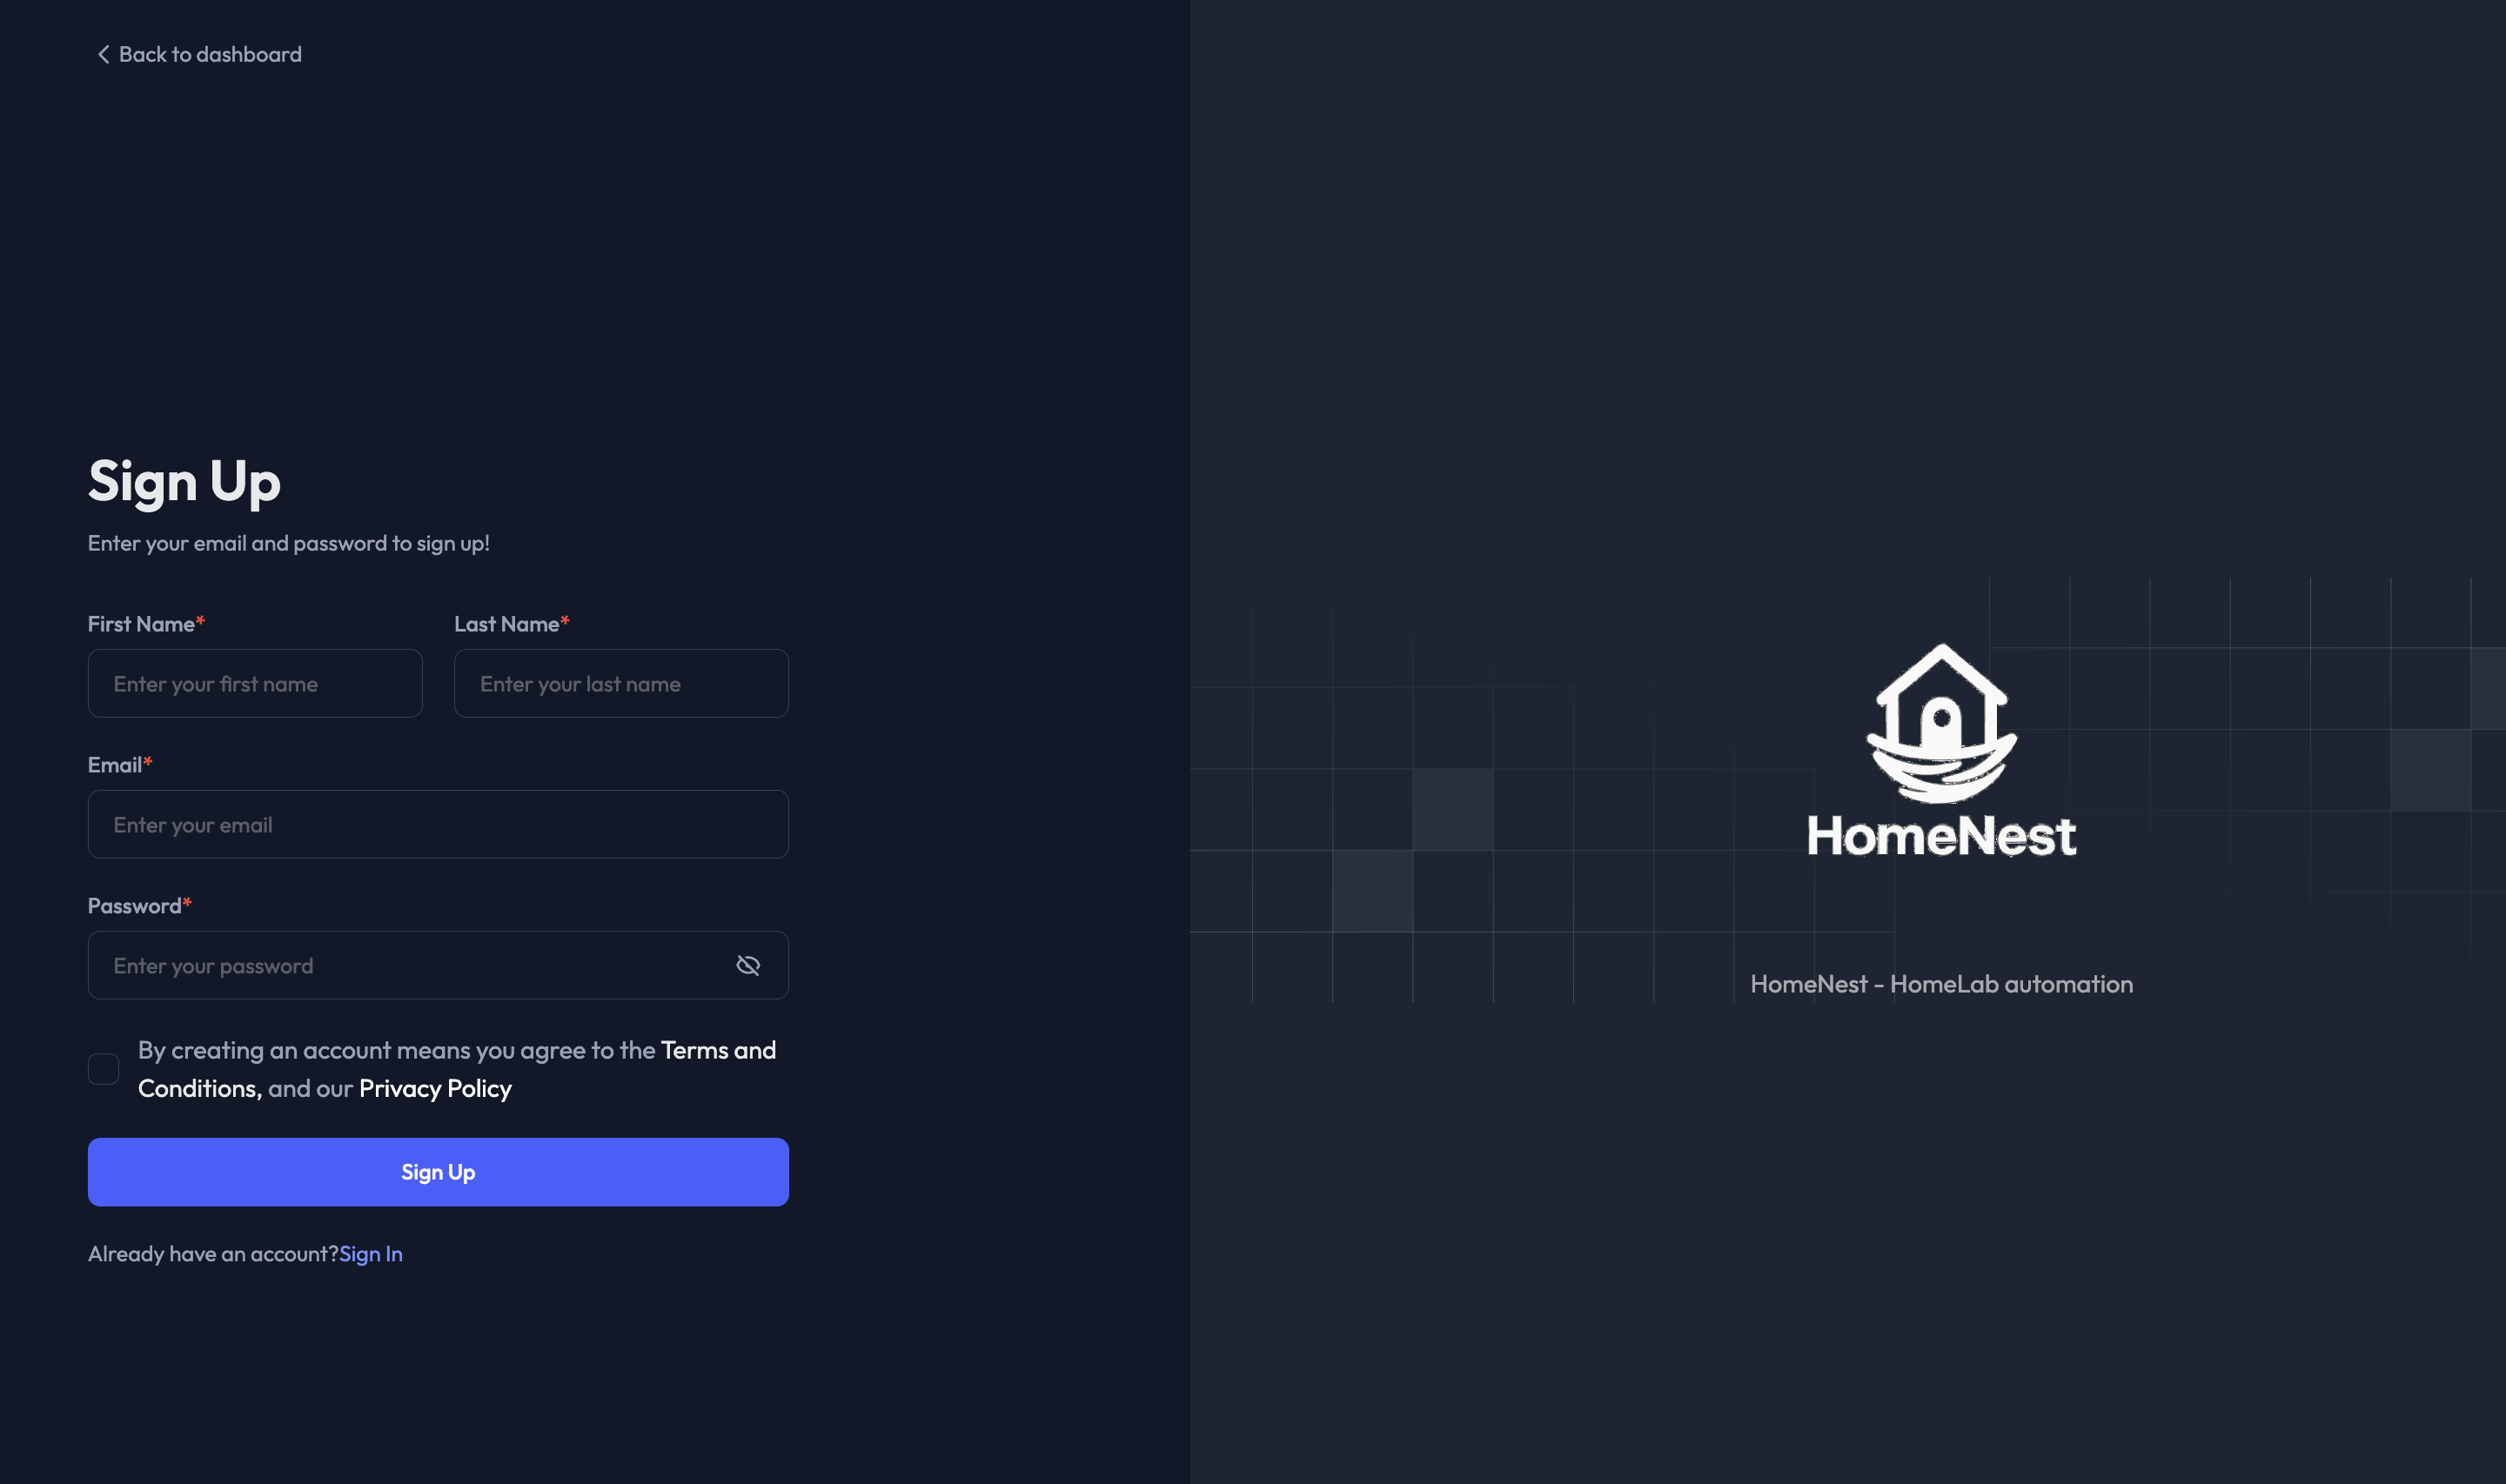
\includegraphics[width=1\textwidth]{./chapters/assets/signup_page.png}
  \caption{Strona Rejestracji do serwisu wyświetlająca logo oraz pola do wprowadzenia danych rejestracji}
  \label{fig:ui_signup}
\end{figure}
Użytkownik może się w tym miejscu zalogować lub zarejestrować przy pomocy adresu email oraz hasła. Rejestracja wymaga podania również swojego imienia i nazwiska oraz zaakceptowania polityk korzystania z serwisu, które będą dodane w późniejszym etapie rozwoju aplikacji.
Możliwa jest również zmiana kolorystyki poprzez naciśnięcie przycisku w prawym dolnym rogu ekranu, co spowoduje zmianę motywu z jasnego na ciemny lub przeciwnie.

\paragraph{Strona przedstawienia oraz integracji Serwisów} - Strona pokazuje obecnie dodane serwisy dostępne w systemie. Umożliwia dodanie własnego serwisu, uruchomienie lub zatrzymanie go oraz przejście do strony HTTP serwisu.
\begin{figure}[H]
  \centering
  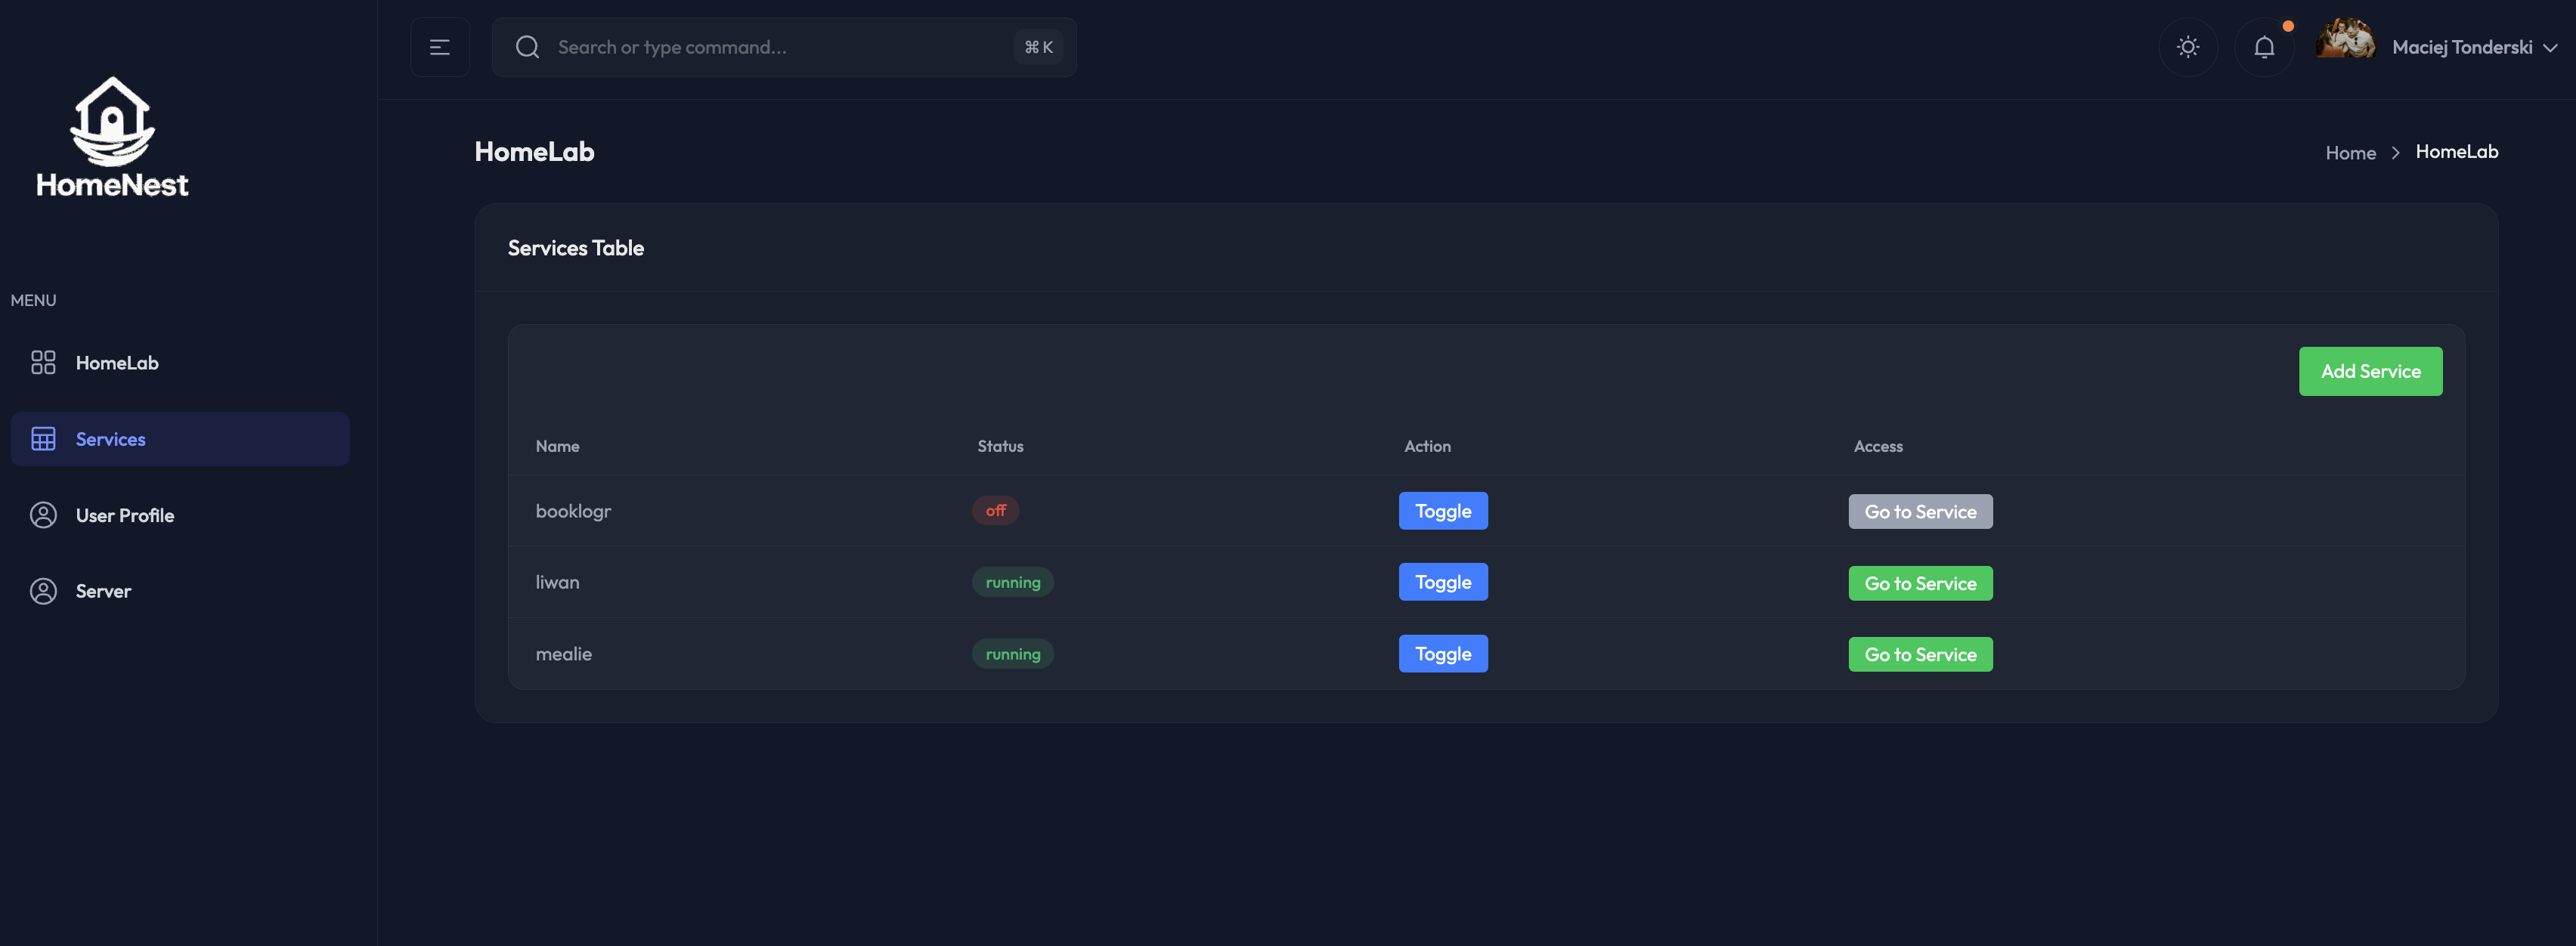
\includegraphics[width=1\textwidth]{./chapters/assets/services_page.png}
  \caption{Podstrona aplikacji odpowiedzialna za wyświetlanie stanu obecnie uruchomionych aplikacji, pozwalająca na ich zarządzanie oraz przekierowująca użytkownika do serwisu.}
  \label{fig:ui_servicespage}
\end{figure}

\paragraph{Strona profilu użytkownika}\mbox{}\\
Strona przedstawia dane użytkownika oraz umożliwia ich edycję. Użytkownik może zmienić swoje imię, nazwisko oraz zdjęcie profilowe. Możliwe jest również wylogowanie się z systemu.

\begin{figure}[H]
  \centering
  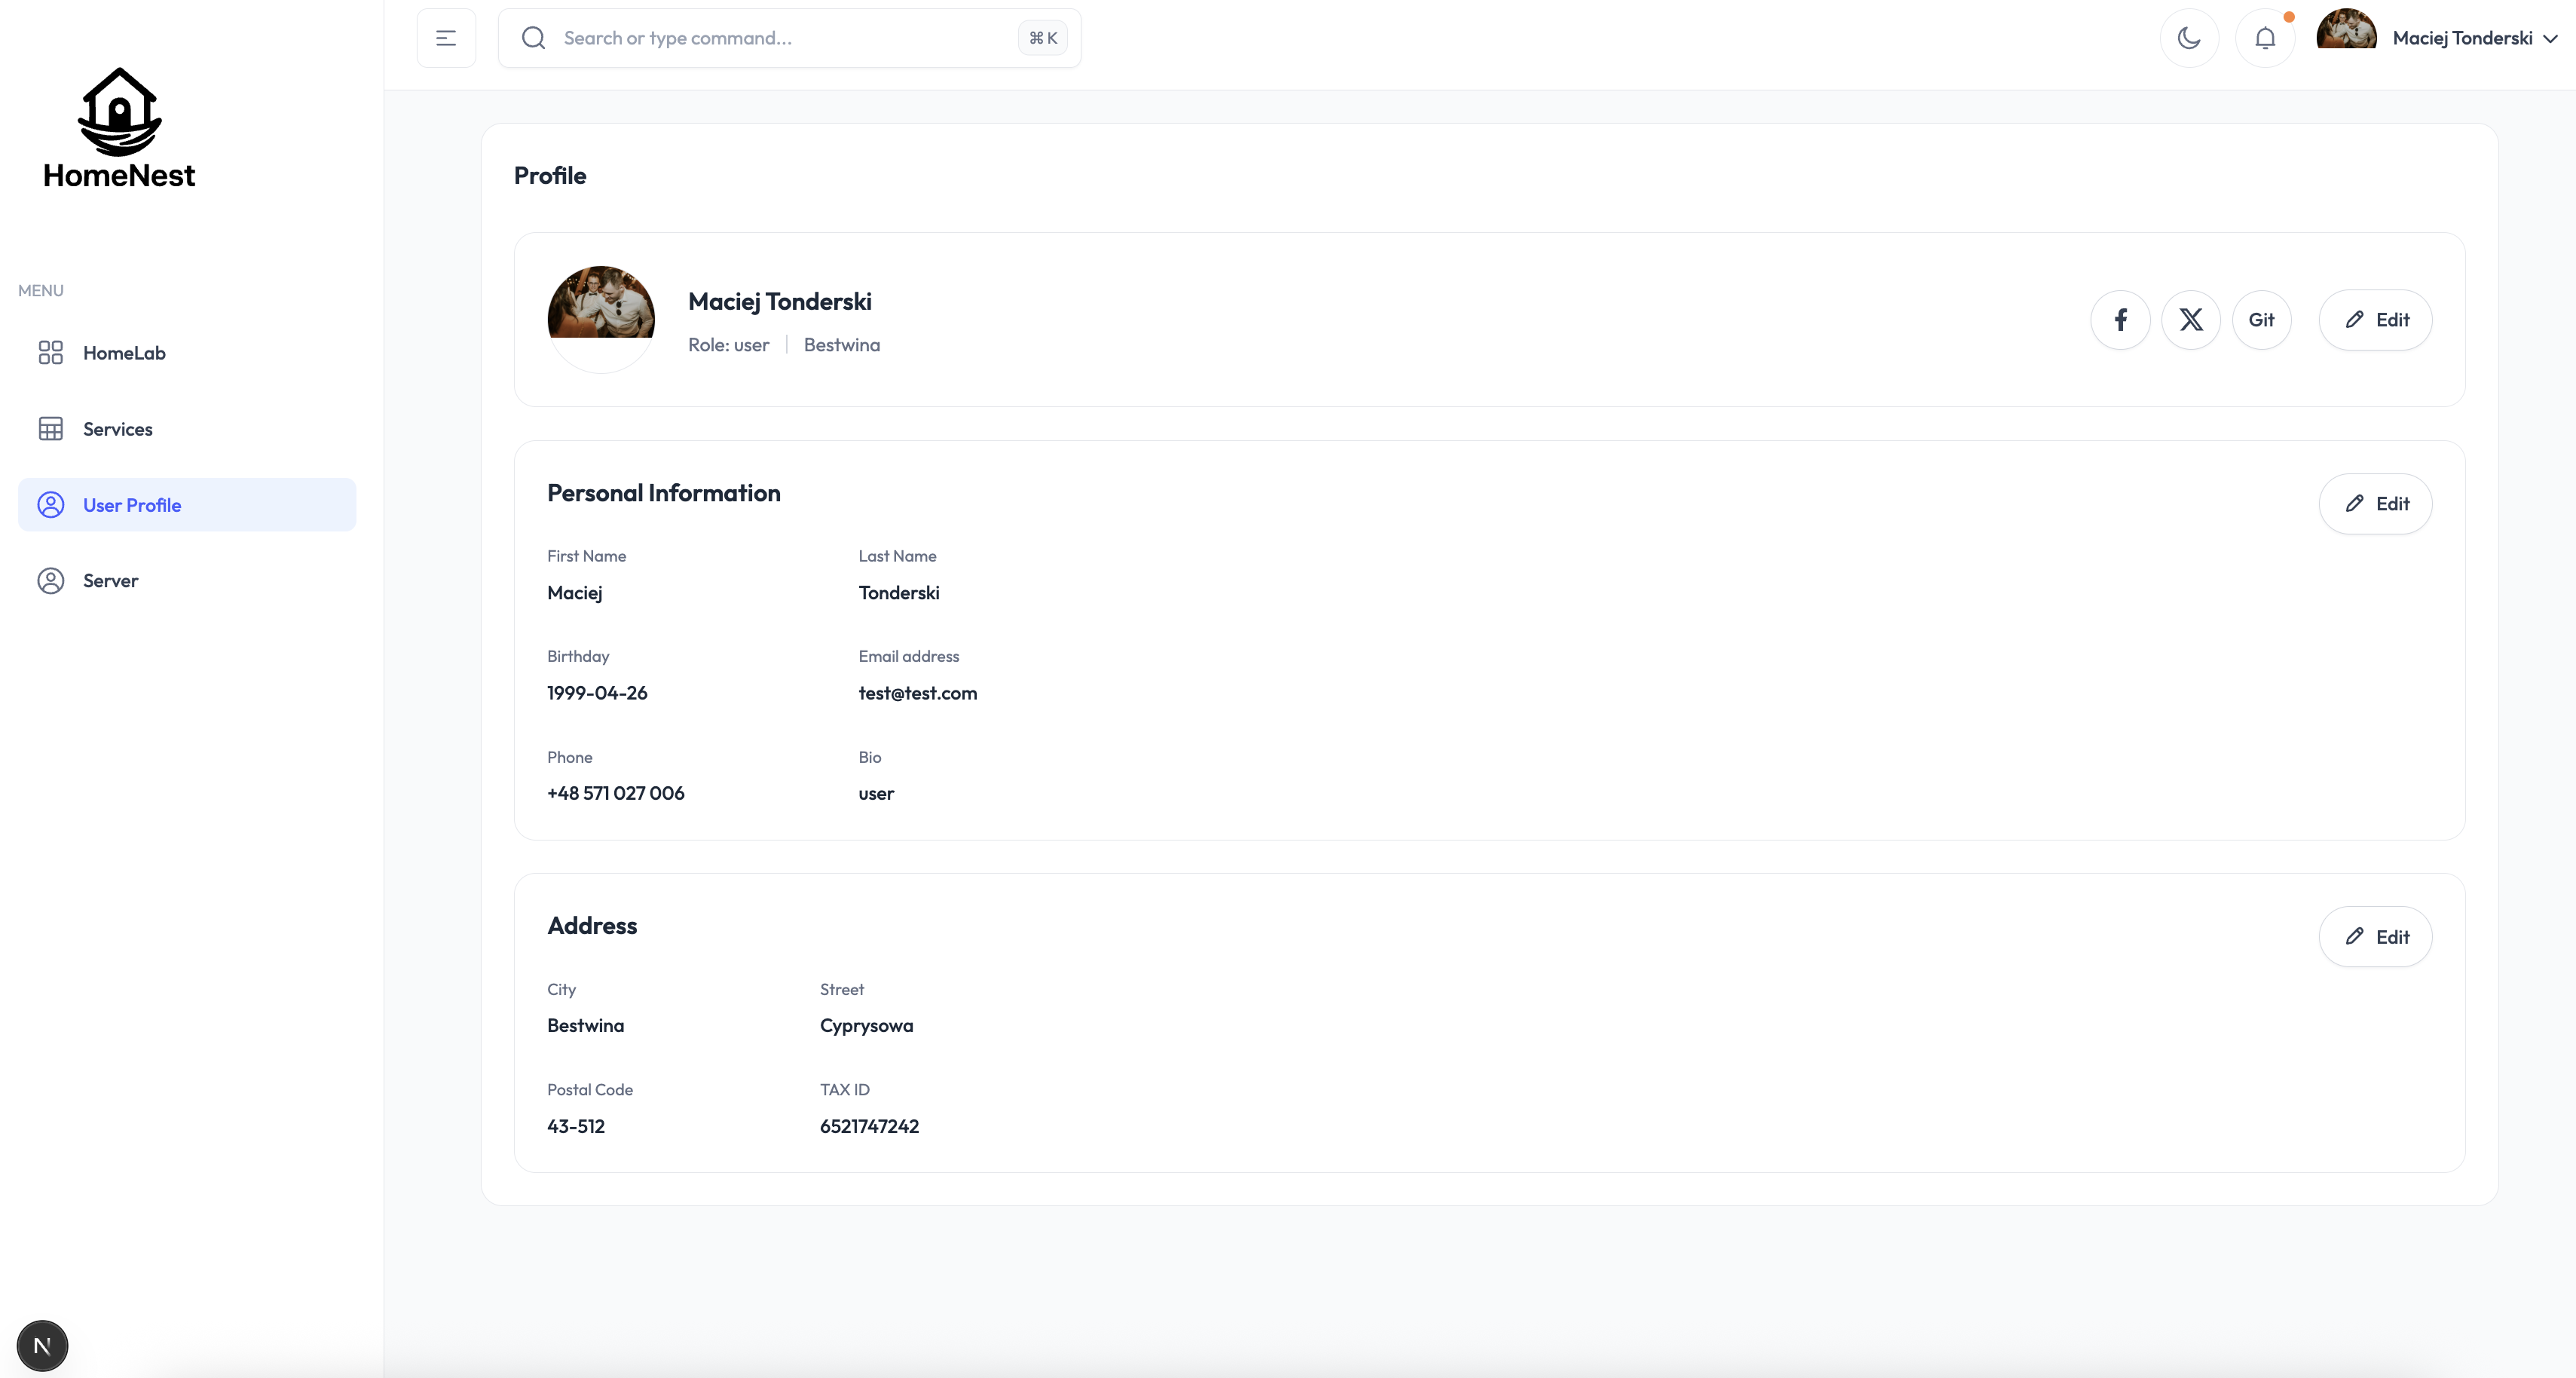
\includegraphics[width=1\textwidth]{./chapters/assets/profile_page.png}
  \caption{Podstrona aplikacji odpowiedzialna za wyświetlanie stanu obecnie uruchomionych aplikacji, pozwalająca na ich zarządzanie oraz przekierowująca użytkownika do serwisu.}
  \label{fig:ui_profile_page}
\end{figure}

\paragraph{Strona zarządzania serwerem}\mbox{}\\

Strona została zaprojektowana z myślą o administratorach systemu, zapewniając im intuicyjne komendy zarządzania serwerem oraz monitorowania jego wydajności i stabilności.

\begin{figure}[H]
  \centering
  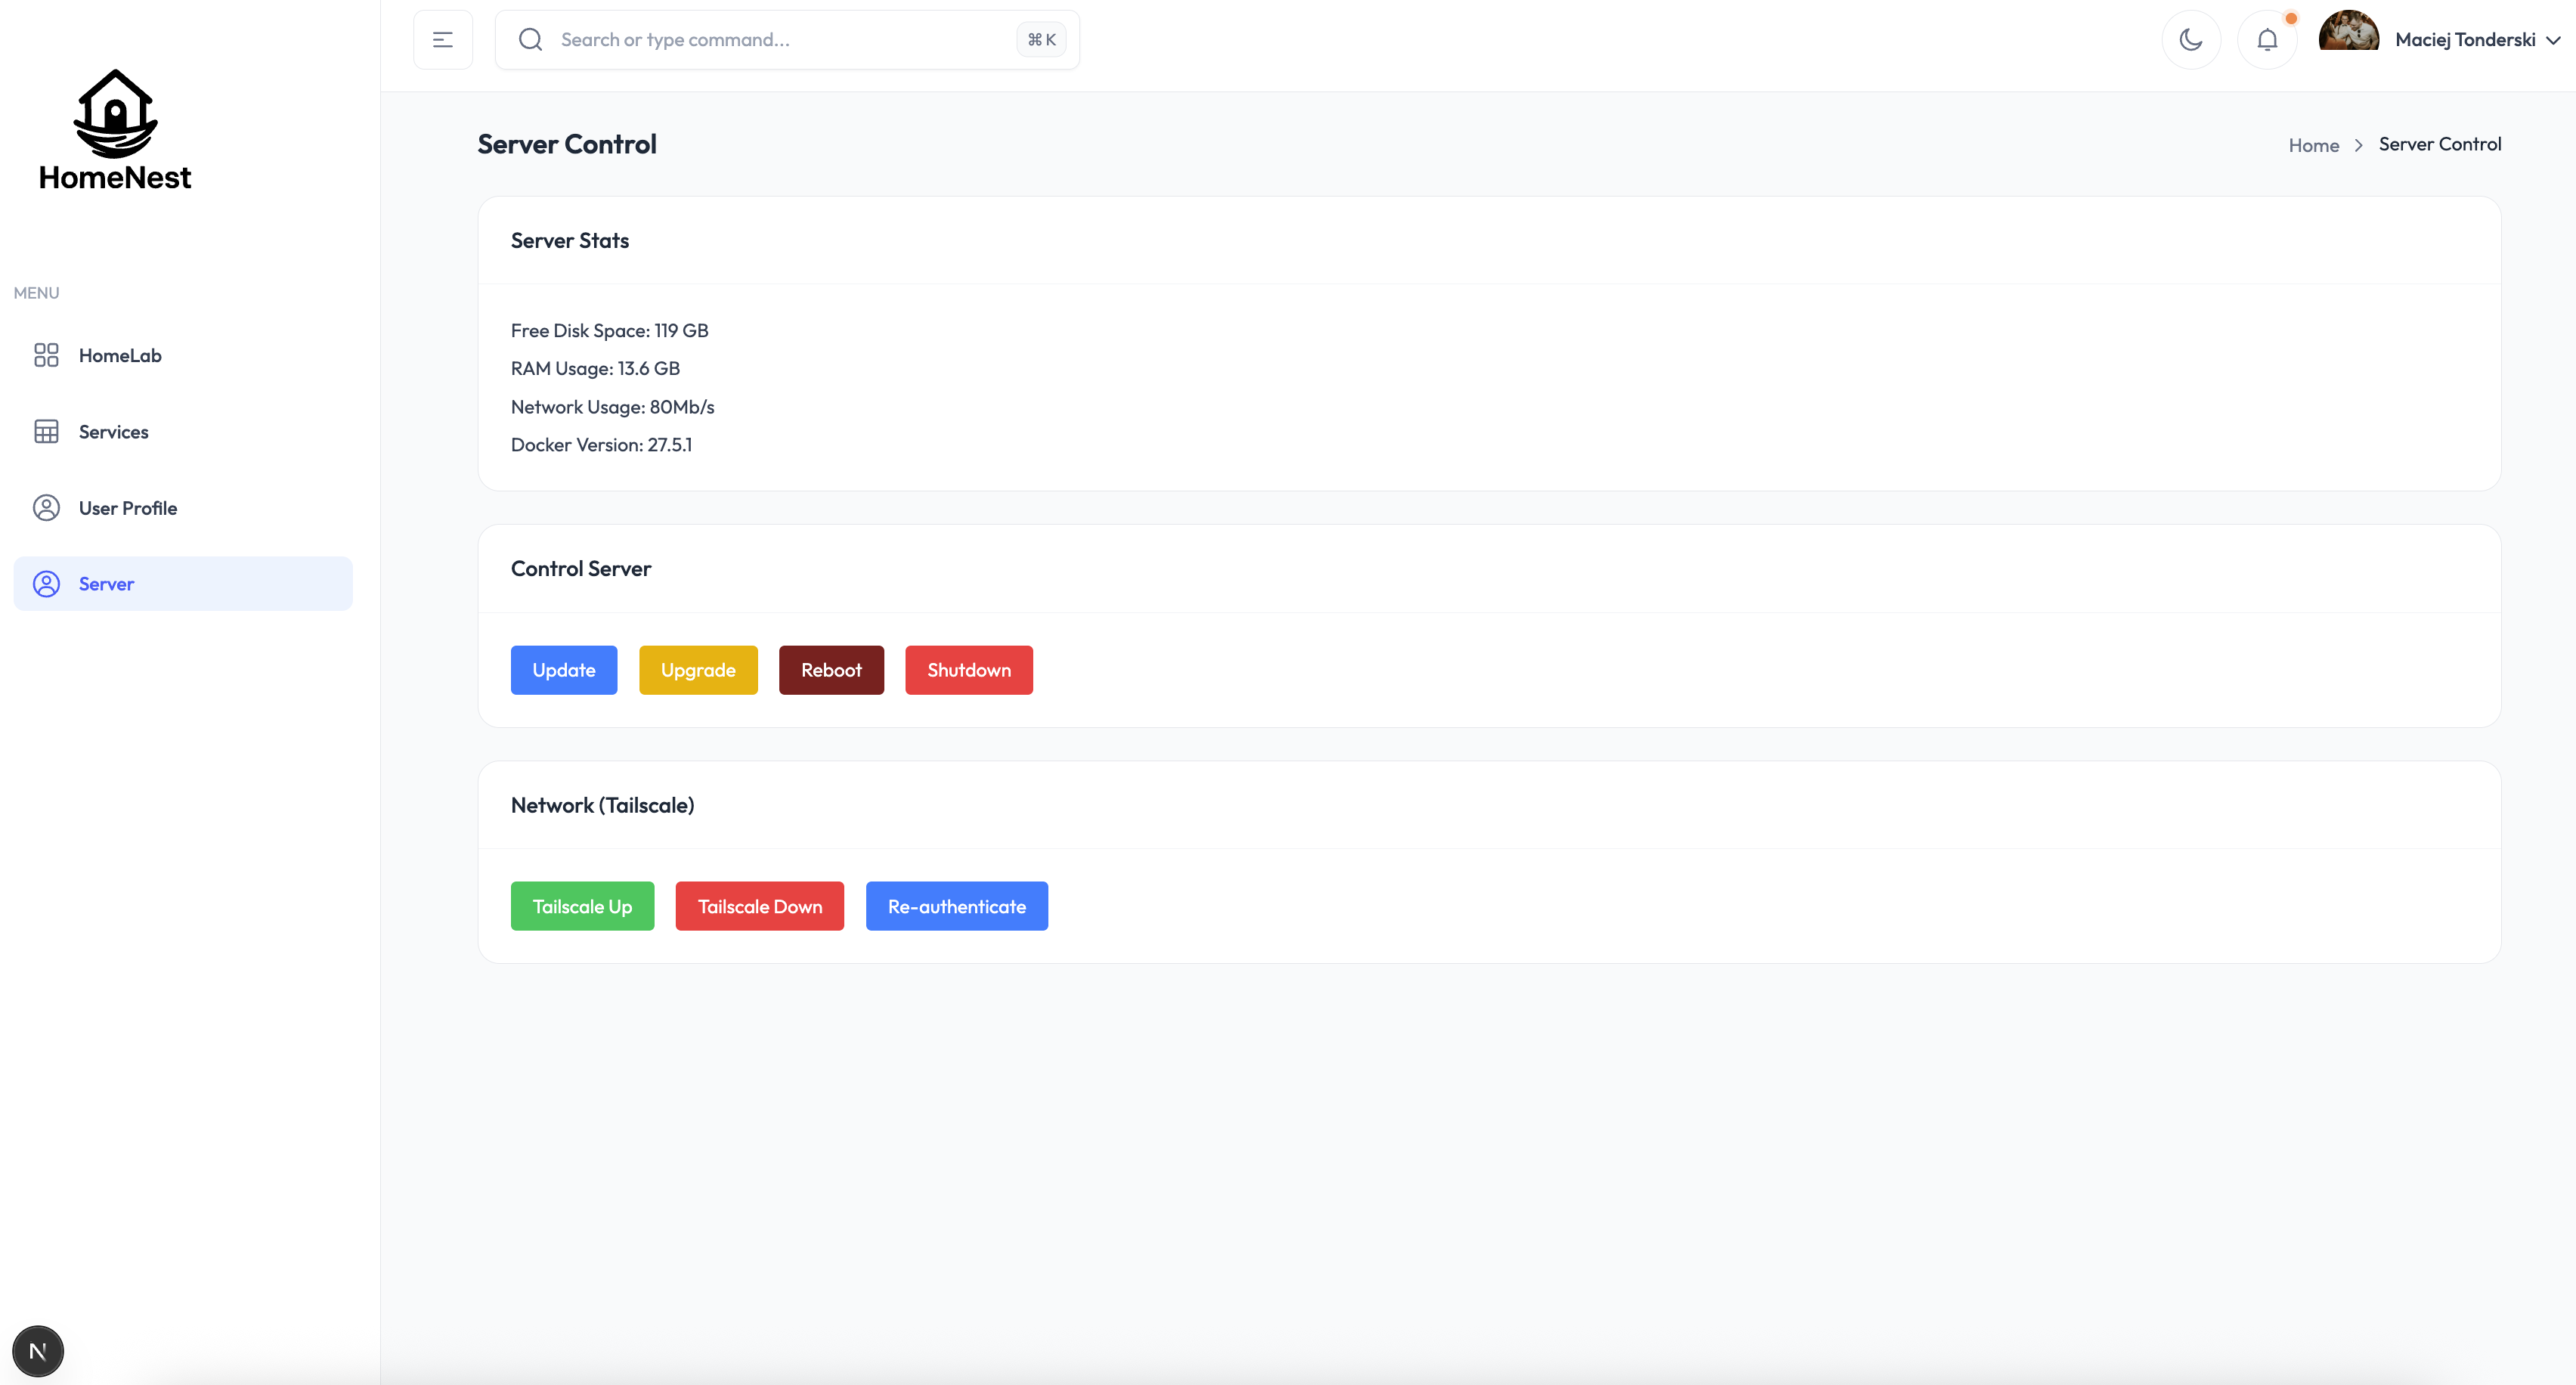
\includegraphics[width=1\textwidth]{./chapters/assets/server_page.png}
  \caption{Podstrona wyświetlająca informacje o stanie serwera, jego zasobach oraz umożliwiająca zarządzanie nimi.}
  \label{fig:ui_server_page}
\end{figure}

\subsubsection{Kolorystyka i typografia}
Projekt interfejsu użytkownika aplikacji HomeNest wykorzystuje nowoczesną i spójną kolorystykę opartą na jasnym tle oraz delikatnych akcentach kolorystycznych. Dominującą barwą tła jest biel (\#ffffff), która nadaje przejrzystości oraz zapewnia wysoki kontrast względem elementów graficznych i tekstu.

Główne akcenty kolorystyczne w interfejsie stanowią odcienie niebieskiego (\#465fff, \#0ba5ec) wykorzystywane m.in. w wykresach, przyciskach akcji oraz wskaźnikach postępu. Barwy te pełnią funkcję informacyjną i nawigacyjną, kierując uwagę użytkownika na istotne elementy interfejsu. Kolorystyka została dodatkowo uzupełniona o neutralne odcienie szarości (\#667085, \#344054), które służą jako tło dla ikon, ramek i tekstów pomocniczych, umożliwiając ich subtelne wydzielenie bez nadmiernego rozpraszania użytkownika.

Zastosowana typografia oparta jest na nowoczesnym, bezszeryfowym kroju pisma, takim jak Outfit, który zapewnia wysoką czytelność niezależnie od rozdzielczości ekranu. Teksty nagłówków oraz wartości liczbowych zostały wyróżnione większym rozmiarem i wzmocnioną wagą fontu (font-medium, font-bold), co wspiera hierarchizację treści. Z kolei opisy pomocnicze oraz etykiety elementów interfejsu zostały zaprezentowane mniejszym rozmiarem i lżejszą barwą, dzięki czemu nie dominują wizualnie nad informacjami kluczowymi.

Zarówno kolorystyka, jak i typografia wspólnie tworzą minimalistyczny, intuicyjny interfejs, dostosowany do długotrwałego użytkowania oraz zgodny z aktualnymi standardami projektowania systemów zarządzania.

Aplikacja HomeNest wspiera również ciemny motyw interfejsu, co zostało zaprezentowane na rysunku poniżej. W tym trybie dominującym kolorem tła jest głęboka barwa granatowo-grafitowa (\#0c111d do \#1d2939), która w połączeniu z jasnymi akcentami (np. odcienie niebieskiego i bieli) zapewnia wysoki kontrast oraz elegancki, nowoczesny wygląd interfejsu.

Elementy interaktywne, jak przyciski czy wykresy, zachowują swoją kolorystykę, jednak są odpowiednio dostosowane do ciemnego tła - np. niebieskie słupki w wykresie API Calls, czy wskaźnik użycia dysku są wyraźnie widoczne również w warunkach ograniczonego oświetlenia.

Typografia w trybie ciemnym pozostaje spójna — fonty bezszeryfowe o wysokiej czytelności są renderowane z jasnymi odcieniami (\#ffffff, \#98a2b3), co sprzyja redukcji zmęczenia wzroku podczas pracy wieczorowej lub w zaciemnionym otoczeniu.

\paragraph{Korzyści wynikające z obsługi dwóch motywów kolorystycznych}\mbox{}\\

Zaprojektowanie interfejsu w dwóch wersjach — jasnej i ciemnej — jest coraz częściej stosowaną praktyką w nowoczesnych aplikacjach webowych i mobilnych. Taka decyzja projektowa niesie ze sobą szereg korzyści:
\begin{itemize}
  \item Dostosowanie do preferencji użytkownika
  Użytkownicy mają różne preferencje dotyczące komfortu pracy z interfejsem. Niektórzy wolą jasne motywy, które przypominają papier i są czytelne w jasnym otoczeniu. Inni preferują ciemne tryby, szczególnie wieczorem, gdy ograniczają zmęczenie wzroku i minimalizują emisję światła niebieskiego.
  \item Lepsze doświadczenie w różnych warunkach oświetleniowych
  Tryb jasny jest bardziej funkcjonalny w warunkach dziennego oświetlenia, natomiast tryb ciemny sprawdza się lepiej przy słabym świetle, np. podczas pracy nocą lub w pomieszczeniach bez dostępu do światła dziennego.
  \item Efektywność energetyczna (w przypadku ekranów OLED)
  W urządzeniach z ekranami OLED tryb ciemny może realnie wpłynąć na oszczędność energii, gdyż piksele wyświetlające kolor czarny są całkowicie wyłączone.
  \item Nowoczesny wygląd aplikacji
  Obsługa trybu ciemnego jest standardem UX w aplikacjach klasy premium i znacząco wpływa na odbiór estetyczny systemu, co może mieć pozytywne znaczenie marketingowe i wizerunkowe.
\end{itemize}


\subsection{Implementacja interfejsu użytkownika}

Interfejs użytkownika aplikacji HomeNest został zaimplementowany w oparciu o gotowy szablon \textbf{TailAdmin}, który dostępny jest publicznie na licencji \textbf{MIT}. TailAdmin to nowoczesny szablon frontendowy oparty na technologii \textbf{React.js}, zbudowany przy użyciu frameworka \textbf{Next.js} oraz systemu stylów \textbf{Tailwind CSS}. Dzięki otwartej licencji możliwe było swobodne dostosowanie szablonu do potrzeb aplikacji oraz jego dalszy rozwój.

\subsubsection{Proces dostosowania szablonu}
W ramach prac wdrożeniowych wykonano następujące kroki:
\begin{enumerate}
    \item \textbf{Pobranie i uruchomienie szablonu} - Skonfigurowano środowisko developerskie oraz uruchomiono projekt TailAdmin w trybie deweloperskim.
    \item \textbf{Dostosowanie struktury aplikacji} - Zmodyfikowano układ nawigacji, menu, system routingu oraz strukturę stron zgodnie z architekturą systemu HomeNest.
    \item \textbf{Implementacja nowych widoków} - Zbudowano dedykowane widoki i komponenty, takie jak: panel główny, zarządzanie usługami, profil użytkownika oraz sekcja administracyjna serwera.
    \item \textbf{Integracja z API backendu} - Komponenty frontendowe zostały zintegrowane z API stworzonym w technologii Go. Dostosowanie szablonu TailAdmin do współpracy z tym API było zadaniem stosunkowo prostym, lecz wymagającym głębszej analizy w celu zoptymalizowania liczby zapytań wykonywanych do backendu oraz zapewnienia wydajnej komunikacji między warstwami systemu.
    \item \textbf{Wprowadzenie trybu ciemnego i jasnego} - Rozbudowano system motywów o możliwość przełączania pomiędzy trybem jasnym i ciemnym, z uwzględnieniem pełnej zgodności stylistycznej.
    \item \textbf{Refaktoryzacja i optymalizacja} - Usunięto zbędne fragmenty kodu, zoptymalizowano komponenty oraz uproszczono logikę interfejsu.
\end{enumerate}

\subsubsection{Zalety podejścia opartego na gotowym szablonie}
\begin{itemize}
    \item Znacząco skrócony czas implementacji frontendowej,
    \item Wysoka jakość kodu źródłowego i zgodność ze standardami branżowymi,
    \item Responsywne komponenty i nowoczesny design,
    \item Możliwość pełnej modyfikacji dzięki licencji MIT,
    \item Spójność wizualna i łatwość integracji z backendem.
\end{itemize}

\subsubsection{Wyzwania podczas adaptacji szablonu}
\begin{itemize}
    \item Konieczność analizy i zrozumienia istniejącej struktury projektu TailAdmin,
    \item Ręczne usuwanie niepotrzebnych widoków i kodu demonstracyjnego,
    \item Potrzeba dostosowania gotowych komponentów do wymagań aplikacji HomeNest,
    \item Zachowanie spójności wizualnej po wprowadzeniu nowych funkcjonalności.
\end{itemize}

Podsumowując, wykorzystanie TailAdmin jako szablonu bazowego pozwoliło na szybkie uruchomienie estetycznego i funkcjonalnego interfejsu użytkownika, a dzięki jego modularności i elastyczności możliwe było skuteczne dostosowanie go do specyfiki systemu HomeNest.


\section{Automatyzacja Konfiguracji i wdrozenie}

\subsection{Instalacja rozwiązania}
W ramach tworzenia rozwiązania powstał również program instalacyjny, który zostanie umieszczony na stronie internetowej rozwiązania umożliwiając pobranie przez zainteresowane korzystaniem z rozwiązania osoby.
\paragraph{Program instalacyjny}\mbox{}\\

W celu ułatwienia instalacji aplikacji na systemach użytkowników końcowych przygotowano dedykowany program instalacyjny napisany w języku Go. Aplikacja ta jest odpowiedzialna za:

\begin{itemize}
    \item Weryfikację obecności Dockera w systemie,
    \item Automatyczną instalację Dockera w systemach Linux (w pozostałych przypadkach użytkownik zostaje poinformowany o konieczności ręcznej instalacji),
    \item Pobranie najnowszej wersji aplikacji HomeNest z repozytorium GitHub,
    \item Rozpakowanie archiwum ZIP zawierającego aplikację do wskazanego katalogu,
    \item Nadanie odpowiednich uprawnień do uruchomienia aplikacji oraz jej uruchomienie.
\end{itemize}

Program wykorzystuje standardowe biblioteki Go do obsługi pobierania plików (\texttt{net/http}), rozpakowywania archiwów ZIP (\texttt{archive/zip}) oraz uruchamiania procesów lokalnych (\texttt{os/exec}). Dzięki temu działa w pełni samodzielnie, bez konieczności instalowania zewnętrznych zależności.

Logika działania programu obejmuje:
\begin{enumerate}
    \item Sprawdzenie czy polecenie \texttt{docker} znajduje się w ścieżce systemowej.
    \item Jeżeli Docker nie jest zainstalowany — uruchomienie skryptu instalacyjnego (tylko w systemach Linux).
    \item Pobranie pliku ZIP z GitHub Releases.
    \item Rozpakowanie pliku do katalogu roboczego.
    \item Uruchomienie pliku binarnego aplikacji.
\end{enumerate}

Instalator został zaprojektowany z myślą o prostocie użytkowania oraz możliwości łatwego wdrożenia aplikacji przez osoby nietechniczne. Wersje programu można przygotować na platformy Linux, Windows i macOS z wykorzystaniem narzędzia \texttt{GOOS/GOARCH}, umożliwiającego cross-kompilację.

\subsection{Integracja z narzędziami CI/CD}
\label{sec:integracja_ci_cd}

System HomeNest wykorzystuje mechanizmy CI/CD oparte na GitHub Actions w celu automatyzacji kluczowych procesów programistycznych — testowania, budowania, wersjonowania i publikacji aplikacji. Dzięki integracji z CI/CD możliwe jest zapewnienie ciągłości rozwoju i wysokiej jakości kodu bez potrzeby ręcznego wykonywania zadań wdrożeniowych.

\subsubsection{Schemat działania}

Po każdej zmianie wprowadzonej do głównej gałęzi \texttt{main}, automatycznie uruchamiane są dwa niezależne pipeline'y GitHub Actions:

\begin{enumerate}
    \item \textbf{Pipeline testujący} — weryfikuje jakość i poprawność kodu,
    \item \textbf{Pipeline release’owy} — buduje artefakty i tworzy release.
\end{enumerate}

\subsubsection{Pipeline testujący}

Pipeline testujący pełni funkcję strażnika jakości kodu. W jego ramach uruchamiane są:

\begin{itemize}
    \item \textbf{Linter} — analizuje kod źródłowy pod kątem zgodności ze standardami formatowania i stylu,
    \item \textbf{Testy jednostkowe backendu} — realizowane za pomocą \texttt{go test}.
\end{itemize}

Dzięki automatycznemu uruchamianiu testów możliwe jest wykrycie regresji i błędów już na etapie developmentu, zanim zostaną wprowadzone do środowiska produkcyjnego.

\subsubsection{Pipeline release’owy}

Po pozytywnym zakończeniu testów uruchamiany jest pipeline odpowiedzialny za zbudowanie artefaktów aplikacji oraz ich publikację jako nowego release'u na GitHubie. Proces ten jest realizowany przy pomocy pliku Makefile, który automatyzuje cały proces budowania i pakowania aplikacji. Makefile definiuje następujące cele:

\begin{itemize}
    \item \textbf{build-frontend} – instalacja zależności npm oraz zbudowanie aplikacji frontendowej; pliki wynikowe umieszczane są w katalogu \texttt{backend/static},
    \item \textbf{build-backend} – kompilacja aplikacji backendowej w Go z ustawieniem zmiennych środowiskowych \texttt{GOOS=linux} i \texttt{GOARCH=amd64}; wynikowy binarny plik jest zapisywany w katalogu \texttt{dist},
    \item \textbf{package} – kopiowanie plików frontendowych do katalogu dystrybucji oraz utworzenie archiwum \texttt{homelab.tar.gz},
    \item \textbf{clean} – usunięcie katalogów zbudowanych artefaktów i archiwum,
    \item \textbf{all} – domyślna akcja wykonująca czyszczenie, budowę frontendu i backendu oraz pakowanie.
\end{itemize}

Pipeline GitHub Actions wywołuje polecenie \texttt{make all}, co zapewnia spójność budowy na każdym etapie. Dzięki temu proces tworzenia release’u jest w pełni zautomatyzowany, powtarzalny i prosty do uruchomienia lokalnie.

\subsubsection{Przykładowy workflow GitHub Actions}

W poniższym przykładzie przedstawiono uproszczony workflow GitHub Actions, który wykorzystuje Makefile do budowania wszystkich komponentów systemu — frontend, backend oraz instalator:

\begin{verbatim}
name: Release Build

on:
  push:
    branches: [main]

jobs:
  build:
    runs-on: ubuntu-latest

    steps:
    - name: Checkout repository
      uses: actions/checkout@v4

    - name: Set up Go
      uses: actions/setup-go@v4
      with:
        go-version: '1.21'

    - name: Set up Node.js
      uses: actions/setup-node@v3
      with:
        node-version: '20'

    - name: Install frontend dependencies
      run: cd frontend && npm ci

    - name: Build all components using Makefile
      run: make all

    - name: Build installer binaries
      run: |
        cd instalator
        make prepare
        make all

    - name: Archive release artifacts
      run: |
        mkdir release
        cp dist/homelab release/
        cp -r dist/static release/static
        cp instalator/build/* release/
        tar -czf release.tar.gz -C release .

    - name: Create GitHub Release
      uses: softprops/action-gh-release@v1
      with:
        tag_name: v${{ github.run_number }}
      env:
        GITHUB_TOKEN: ${{ secrets.GITHUB_TOKEN }}
      files: |
        release.tar.gz
\end{verbatim}

\subsubsection{Strategia wersjonowania}

Każdy release oznaczany jest automatycznie na podstawie numeru buildu. W przyszłości możliwe będzie również wdrożenie semantycznego wersjonowania (SemVer) w oparciu o analizę commitów.

\subsubsection{Weryfikacja aktualności aplikacji}

W przyszłości system zostanie rozszerzony o mechanizm, który cyklicznie będzie odpytywał GitHub API w celu sprawdzenia dostępności nowego release’u. Porównując aktualnie zainstalowaną wersję z najnowszym tagiem, system będzie w stanie:

\begin{itemize}
    \item Powiadomić użytkownika o dostępnej aktualizacji,
    \item Wyświetlić changelog (opis zmian z release notes),
    \item Zaproponować pobranie i automatyczne wdrożenie nowej wersji.
\end{itemize}

Taka funkcjonalność przyczyni się do utrzymania systemu w najnowszej, stabilnej wersji bez potrzeby ręcznej ingerencji.

\subsubsection{Korzyści z automatyzacji CI/CD}

Integracja GitHub Actions pozwala na:

\begin{itemize}
    \item Skrócenie czasu wdrożeń,
    \item Unifikację procesu testowania i publikacji,
    \item Eliminację błędów ludzkich,
    \item Wzrost zaufania do jakości aplikacji,
    \item Łatwą replikację procesu na nowych środowiskach (np. staging, produkcja).
\end{itemize}

Dzięki powyższym cechom proces CI/CD jest nieodzownym elementem systemu HomeNest i fundamentem jego dalszego skalowania.
\chapter{Testowanie i analiza systemu}

\section{Testy jednostkowe i integracyjne}
Testowanie oprogramowania jest kluczowym elementem zapewnienia jego jakości, stabilności i niezawodności. W ramach niniejszej pracy zastosowano zarówno testy jednostkowe, jak i testy integracyjne w celu weryfikacji poprawności działania poszczególnych modułów systemu oraz ich wzajemnych interakcji.

\subsection{Testy jednostkowe}

Testy jednostkowe koncentrują się na sprawdzaniu poprawności działania pojedynczych funkcji i metod w izolacji. Ich głównym celem jest szybkie wykrywanie błędów w logice aplikacji oraz zapewnienie, że każdy komponent działa zgodnie z oczekiwaniami. W testowaniu jednostkowym zastosowano bibliotekę \textbf{pytest} oraz narzędzie \textbf{unittest} w Pythonie.

Przykładowe testy jednostkowe obejmowały:
\begin{itemize}
    \item Sprawdzenie poprawności działania funkcji hashującej hasła użytkowników,
    \item Weryfikację generowania i walidacji tokenów JWT,
    \item Testy funkcji odpowiedzialnych za zarządzanie użytkownikami (dodawanie, edycja, usuwanie),
    \item Weryfikację poprawności operacji CRUD dla bazy danych MongoDB.
\end{itemize}

Wszystkie testy jednostkowe zostały zautomatyzowane i uruchamiane w ramach procesu CI/CD z wykorzystaniem GitHub Actions oraz samodzielnie hostowanych runnerów.

\subsection{Testy integracyjne}

Testy integracyjne mają na celu sprawdzenie współpracy różnych komponentów systemu, takich jak API, baza danych oraz interfejs użytkownika. W ramach pracy przeprowadzono testy integracyjne z użyciem frameworka \textbf{pytest} wraz z modułem \textbf{httpx}, umożliwiającym wysyłanie zapytań HTTP do testowanego serwera.

Zakres testów integracyjnych obejmował:
\begin{itemize}
    \item Sprawdzenie poprawności obsługi żądań API przez FastAPI,
    \item Testy poprawności integracji systemu uwierzytelniania JWT z bazą danych,
    \item Weryfikację działania operacji na usługach, takich jak rejestrowanie, uruchamianie i zatrzymywanie kontenerów.
\end{itemize}

Testy integracyjne zostały przeprowadzone zarówno w środowisku lokalnym, jak i w środowisku testowym z wykorzystaniem kontenerów Docker.

\subsection{Podsumowanie testów}

Przeprowadzone testy jednostkowe i integracyjne pozwoliły na wykrycie oraz eliminację potencjalnych błędów na wczesnym etapie rozwoju aplikacji. Dzięki zastosowaniu automatyzacji testów oraz integracji z procesem CI/CD, system został zoptymalizowany pod kątem stabilności i niezawodności. Testowanie stanowiło istotny element procesu wdrażania i potwierdziło poprawność działania kluczowych funkcjonalności systemu HomeLab.

\section{Testy wydajnościowe i bezpieczeństwa}
\subsection{Testowanie wydajności systemu}

Testowanie wydajności aplikacji jest kluczowym elementem zapewnienia jej stabilności i efektywności w warunkach produkcyjnych. W celu przeprowadzenia testów wydajnościowych wykorzystano narzędzie \textbf{Locust}, które pozwala na symulację obciążenia aplikacji przez wielu użytkowników jednocześnie.

\subsubsection{Cel testów wydajnościowych}
Celem testów wydajnościowych było:
\begin{itemize}
    \item Ocena wydajności API w warunkach wysokiego obciążenia,
    \item Pomiar czasu odpowiedzi kluczowych endpointów,
    \item Weryfikacja stabilności systemu podczas długotrwałego obciążenia,
    \item Identyfikacja potencjalnych wąskich gardeł aplikacji.
\end{itemize}

\subsubsection{Metodyka testów}
Testy wydajnościowe przeprowadzono przy użyciu Locust, który pozwala na definiowanie scenariuszy użytkowników wykonujących określone operacje. Wykorzystano następujące kroki:
\begin{enumerate}
    \item Zalogowanie użytkownika i uzyskanie tokena JWT,
    \item Wykonywanie żądań do kluczowych endpointów API (zarządzanie usługami, monitorowanie systemu, operacje administracyjne),
    \item Pomiar czasu odpowiedzi serwera i obciążenia systemu,
    \item Skalowanie liczby użytkowników w celu oceny zachowania systemu pod rosnącym obciążeniem.
\end{enumerate}

\subsubsection{Zakres testów}
W ramach testów wydajnościowych poddano analizie następujące funkcjonalności:
\begin{itemize}
    \item \textbf{Autoryzacja i uwierzytelnianie} – logowanie użytkowników i uzyskiwanie tokenów JWT,
    \item \textbf{Zarządzanie usługami} – pobieranie listy uruchomionych usług, monitorowanie ich stanu oraz restartowanie usług w złym stanie,
    \item \textbf{Monitorowanie systemu} – pobieranie danych dotyczących zużycia CPU, pamięci RAM oraz listy aktywnych kontenerów Docker,
    \item \textbf{Zarządzanie użytkownikami} – dodawanie i listowanie użytkowników.
\end{itemize}

\subsubsection{Wyniki testów}
Po przeprowadzeniu testów otrzymano następujące wyniki:
\begin{itemize}
    \item Średni czas odpowiedzi API dla standardowych żądań wynosił poniżej 70 ms (lokalne środowisko - w tej samej sieci),
    \item Przy zwiększeniu liczby jednocześnie aktywnych użytkowników do 1000 system nadal utrzymywał stabilność, przy wzroście czasu odpowiedzi do około 190 ms,
    \item Największe obciążenie dotyczyło operacji związanych z monitorowaniem systemu, co wynika z konieczności pobierania danych o stanie zasobów w czasie rzeczywistym - wskazuje to na konieczność zastosowania cachowania danych dotyczących stanu systemu celem uniknięcia ataktu DDoS,
    \item Endpointy administracyjne, takie jak restart serwera czy autoryzacja w Tailscale, działały poprawnie, lecz wymagają dodatkowych zabezpieczeń przed wielokrotnym wywołaniem w krótkim czasie.
\end{itemize}

\subsubsection{Wnioski i optymalizacje}
Na podstawie przeprowadzonych testów wydajnościowych zaproponowano następujące optymalizacje:
\begin{itemize}
    \item Implementacja mechanizmu cache'owania dla danych monitorowania systemu w celu zmniejszenia liczby odczytów zasobów,
    \item Ograniczenie liczby jednoczesnych zapytań do endpointów administracyjnych,
    \item Optymalizacja zapytań do bazy danych poprzez indeksowanie często wyszukiwanych pól.
\end{itemize}

Testy wykazały, że system jest w stanie obsłużyć duże obciążenie i zachowuje stabilność przy wysokiej liczbie równoczesnych użytkowników, co potwierdza jego gotowość do wdrożenia w środowisku produkcyjnym.

\subsection{Testowanie bezpieczeństwa aplikacji}

Bezpieczeństwo aplikacji webowych jest kluczowym aspektem zapewnienia poufności, integralności i dostępności danych. Testowanie bezpieczeństwa ma na celu identyfikację potencjalnych luk oraz podatności, które mogą zostać wykorzystane przez nieautoryzowanych użytkowników lub atakujących.

\textbf{Należy zaznaczyć, że w ramach niniejszej pracy magisterskiej testy bezpieczeństwa nie zostały przeprowadzone. Poniższy rozdział ma charakter teoretyczny i przedstawia ogólne zasady oraz metody stosowane w testowaniu bezpieczeństwa aplikacji webowych.}

\subsubsection{Metodyka testowania bezpieczeństwa}
Testowanie bezpieczeństwa można podzielić na kilka kluczowych etapów:
\begin{itemize}
    \item \textbf{Analiza architektury} – Przegląd struktury aplikacji, mechanizmów autoryzacji i uwierzytelniania,
    \item \textbf{Testy penetracyjne} – Symulowane ataki w celu sprawdzenia odporności na znane zagrożenia,
    \item \textbf{Analiza kodu źródłowego} – Poszukiwanie błędów bezpieczeństwa w implementacji aplikacji,
    \item \textbf{Fuzzing} – Automatyczne generowanie losowych danych wejściowych w celu wykrycia awarii,
    \item \textbf{Skany podatności} – Wykorzystanie narzędzi do identyfikacji znanych luk w zabezpieczeniach.
\end{itemize}

\subsubsection{Obszary testowania bezpieczeństwa}
Testowanie bezpieczeństwa aplikacji obejmuje następujące obszary:

\paragraph{1. Uwierzytelnianie i autoryzacja}
Mechanizmy uwierzytelniania powinny być odporne na ataki brute-force oraz przechowywać hasła w bezpieczny sposób. Kluczowe testy obejmują:
\begin{itemize}
    \item Testowanie siły haseł i polityki logowania,
    \item Próby ataków brute-force na endpointy logowania,
    \item Weryfikacja poprawności implementacji JWT i zarządzania sesjami,
    \item Sprawdzenie uprawnień użytkowników do zasobów.
\end{itemize}

\paragraph{2. Zarządzanie danymi i ochrona przed SQL Injection}
Baza danych powinna być zabezpieczona przed atakami wstrzykiwania SQL. Weryfikacja obejmuje:
\begin{itemize}
    \item Testy podatności na SQL Injection przy użyciu specjalnie spreparowanych zapytań,
    \item Sprawdzenie, czy aplikacja korzysta z mechanizmów ORM i zapytań parametryzowanych,
    \item Ograniczenie uprawnień użytkowników bazy danych.
\end{itemize}

\paragraph{3. Ochrona przed atakami XSS i CSRF}
Ataki Cross-Site Scripting (XSS) i Cross-Site Request Forgery (CSRF) mogą prowadzić do przejęcia sesji użytkownika lub wykonania nieautoryzowanych operacji. Testy obejmują:
\begin{itemize}
    \item Wstrzykiwanie skryptów JavaScript w formularzach i żądaniach API,
    \item Weryfikację nagłówków zabezpieczających (Content Security Policy, SameSite Cookies),
    \item Sprawdzenie zabezpieczeń przed atakami CSRF poprzez implementację tokenów anty-CSRF.
\end{itemize}

\paragraph{4. Bezpieczeństwo API}
Bezpieczeństwo API jest kluczowe dla ochrony danych przesyłanych pomiędzy klientem a serwerem. Testowanie obejmuje:
\begin{itemize}
    \item Sprawdzenie poprawności nagłówków autoryzacyjnych,
    \item Testy na ataki replay (ponowne wykorzystanie żądań API),
    \item Weryfikację mechanizmów rate-limiting (ograniczenie liczby żądań w czasie),
    \item Ochronę przed atakami Man-in-the-Middle (MITM) poprzez wymuszanie HTTPS.
\end{itemize}

\paragraph{5. Odporność na ataki DoS/DDoS}
Ataki Denial of Service (DoS) mogą doprowadzić do przeciążenia aplikacji i uniemożliwienia jej działania. Testy obejmują:
\begin{itemize}
    \item Symulację dużej liczby jednoczesnych żądań,
    \item Weryfikację mechanizmów ograniczających dostępność zasobów,
    \item Sprawdzenie konfiguracji serwera pod kątem ochrony przed atakami DDoS.
\end{itemize}

\subsubsection{Narzędzia do testowania bezpieczeństwa}
Do testowania bezpieczeństwa wykorzystuje się różne narzędzia, m.in.:
\begin{itemize}
    \item \textbf{OWASP ZAP} – Automatyczne skanowanie podatności aplikacji webowych,
    \item \textbf{Burp Suite} – Analiza i przechwytywanie ruchu HTTP/HTTPS,
    \item \textbf{sqlmap} – Automatyczne wykrywanie podatności na SQL Injection,
    \item \textbf{Metasploit} – Wykonywanie testów penetracyjnych,
    \item \textbf{Fail2Ban} – Ochrona przed atakami brute-force poprzez blokowanie adresów IP.
\end{itemize}

\subsubsection{Podsumowanie}
Testowanie bezpieczeństwa aplikacji webowych jest kluczowym elementem zapewnienia ochrony danych i usług. Wykorzystanie kompleksowego podejścia, obejmującego testy penetracyjne, analizę kodu oraz automatyczne skanowanie podatności, pozwala na wczesne wykrycie zagrożeń i skuteczne zabezpieczenie systemu przed atakami. Regularne testy i aktualizacje mechanizmów bezpieczeństwa są niezbędne do utrzymania wysokiego poziomu ochrony aplikacji.

\textbf{Podkreśla się, że powyższe informacje mają charakter teoretyczny i w ramach niniejszej pracy magisterskiej nie przeprowadzono rzeczywistych testów bezpieczeństwa aplikacji.}
\chapter{Podsumowanie i wnioski}

\section{Podsumowanie pracy}

W niniejszej pracy magisterskiej przedstawiono projekt, implementację oraz analizę systemu zarządzania usługami i monitorowania serwera, napisanego w języku Go. System składa się z backendu (API) stworzonego w Go oraz frontendowej części zbudowanej w oparciu o szablon TailAdmin. Celem pracy było stworzenie wydajnej i bezpiecznej aplikacji umożliwiającej administratorom zarządzanie usługami systemowymi, monitorowanie wykorzystania zasobów oraz przeprowadzanie operacji administracyjnych na serwerze.

W trakcie realizacji projektu skupiono się na kilku kluczowych aspektach, w tym implementacji API w Go, integracji z interfejsem użytkownika TailAdmin, zarządzaniu użytkownikami, optymalizacji wydajności oraz aspektach związanych z bezpieczeństwem aplikacji webowych. Każdy z tych elementów został szczegółowo opisany i przeanalizowany, co pozwoliło na wyciągnięcie cennych wniosków dotyczących zarówno języka Go, jak i nowoczesnych narzędzi frontendowych i backendowych stosowanych w zarządzaniu infrastrukturą IT.

Instrukcja instalacji oraz uruchomienia aplikacji została zamieszczona w pliku \texttt{README.md} w repozytorium projektu na platformie GitHub\cite{NestOpsV2}.


\subsection{Osiągnięcia i rezultaty pracy}

W ramach realizacji pracy magisterskiej osiągnięto szereg istotnych rezultatów, które potwierdzają praktyczną użyteczność oraz skalowalność zaprojektowanego systemu. Najważniejsze z nich to:

\begin{itemize}
    \item Zaprojektowano oraz zaimplementowano backend systemu przy użyciu języka Go. Dzięki zastosowaniu tej technologii aplikacja cechuje się wysoką wydajnością, prostotą dystrybucji oraz łatwością utrzymania.
    \item Opracowano nowoczesny, responsywny interfejs użytkownika wykorzystując szablon TailAdmin. Interfejs ten umożliwia intuicyjne zarządzanie usługami systemowymi i użytkownikami, a także prezentuje dane o stanie systemu w przejrzystej formie.
    \item Stworzono kompletne REST API umożliwiające zarządzanie użytkownikami, usługami oraz monitorowanie parametrów systemowych. API zostało zaprojektowane w sposób modularny i rozszerzalny.
    \item Wdrożono mechanizmy uwierzytelniania i autoryzacji użytkowników z wykorzystaniem JWT. System obsługuje różne poziomy uprawnień oraz zabezpiecza dostęp do krytycznych funkcjonalności.
    \item Zaimplementowano funkcjonalności administracyjne obejmujące dodawanie, edytowanie, usuwanie i przeglądanie użytkowników z poziomu panelu administratora.
    \item Umożliwiono rejestrowanie i zarządzanie usługami systemowymi – uruchamianie, zatrzymywanie oraz monitorowanie ich stanu w czasie rzeczywistym.
    \item Zintegrowano backend z systemem operacyjnym w zakresie kontroli nad aktywnymi usługami systemowymi i dostępem do danych o zużyciu zasobów (RAM, CPU, dysk).
    \item Przeprowadzono testy wydajnościowe z użyciem narzędzia Ddosify, które wykazały odporność aplikacji na duże obciążenia oraz pomogły zidentyfikować krytyczne momenty wymagające optymalizacji.
    \item Zrealizowano testy bezpieczeństwa, w tym odporności na ataki typu brute-force, dostęp nieautoryzowany, SQL Injection oraz Cross-Site Scripting, potwierdzając bezpieczeństwo podstawowych mechanizmów aplikacji.
    \item Opracowano system budowania i pakowania aplikacji za pomocą Makefile, umożliwiający łatwą kompilację na wiele platform oraz automatyczne tworzenie paczek instalacyjnych.
    \item Udokumentowano projekt w postaci pliku \texttt{README.md} na GitHubie, w którym zawarto instrukcję instalacji, konfiguracji i uruchomienia systemu zarówno na lokalnych maszynach, jak i w środowiskach produkcyjnych.
\end{itemize}

System powstały w wyniku realizacji pracy magisterskiej został zaprojektowany zgodnie z zasadami czystej architektury i modularności, co pozwala na jego dalsze rozwijanie i dostosowywanie do indywidualnych potrzeb użytkowników oraz specyfiki środowiska produkcyjnego. Aktualna wersja spełnia wszystkie założenia funkcjonalne, stanowiąc stabilną podstawę dla rzeczywistego wdrożenia.

\subsection{Wnioski i przyszłe kierunki rozwoju}

Na podstawie przeprowadzonych badań, testów oraz implementacji można sformułować następujące wnioski:

\begin{itemize}
    \item Połączenie języka Go w warstwie backendu oraz szablonu TailAdmin w warstwie frontendowej pozwala na szybkie tworzenie aplikacji o wysokiej wydajności i przejrzystym interfejsie użytkownika.
    \item Architektura systemu została zaprojektowana w sposób umożliwiający jego łatwą rozbudowę – zarówno poprzez dodawanie nowych endpointów API, jak i integrację z zewnętrznymi usługami.
    \item Testy wydajnościowe ujawniły, że system dobrze radzi sobie z typowym obciążeniem, jednak należy zwrócić uwagę na ograniczenia wynikające z zastosowania SQLite, szczególnie przy dużej liczbie jednoczesnych operacji zapisu.
    \item Mechanizmy bezpieczeństwa wdrożone w systemie (autoryzacja JWT, kontrola ról, odporność na podstawowe ataki webowe) są wystarczające na etapie prototypowania, jednak wymagają dalszej rozbudowy przed wdrożeniem produkcyjnym.
\end{itemize}

W przyszłości system może zostać rozszerzony o:

\begin{itemize}
    \item Wdrożenie kolejki zadań (np. z użyciem Redis lub RabbitMQ) w celu obsługi operacji asynchronicznych oraz przetwarzania zadań wymagających więcej czasu.
    \item Rozszerzenie API o nowe funkcjonalności, takie jak integracja z narzędziami CI/CD, mechanizmy webhooków, czy eksport danych do zewnętrznych systemów.
    \item Zastosowanie bazy danych wspierającej jednoczesne zapisy (np. PostgreSQL) dla zwiększenia skalowalności.
    \item Integrację z narzędziami monitorującymi (np. Prometheus, Grafana) i systemami SIEM w celu zwiększenia widoczności operacyjnej i poziomu bezpieczeństwa.
    \item Wprowadzenie funkcjonalności cache’owania danych, aby zmniejszyć obciążenie backendu i przyspieszyć odpowiedzi aplikacji.
    \item Wdrożenie mechanizmów uwierzytelniania wieloskładnikowego (MFA) oraz integrację z zewnętrznymi systemami tożsamości (np. LDAP, OAuth).
\end{itemize}

Podsumowując, opracowana aplikacja stanowi solidne i nowoczesne rozwiązanie, które może być wykorzystane zarówno w małych środowiskach serwerowych, jak i jako baza pod rozbudowane systemy administracji IT. Projekt może zostać rozwinięty o nowe funkcje i zintegrowany z narzędziami stosowanymi w profesjonalnym zarządzaniu infrastrukturą informatyczną.


\section{Możliwości dalszego rozwoju systemu}

Opracowany system zarządzania usługami i monitorowania serwera został zaprojektowany w sposób modularny i skalowalny, co pozwala na jego dalszą rozbudowę. Możliwe kierunki rozwoju obejmują zarówno ulepszenia funkcjonalne, jak i wdrożenie zaawansowanych mechanizmów zwiększających wydajność oraz bezpieczeństwo systemu. W niniejszym rozdziale przedstawiono propozycje rozszerzeń, które mogą znacząco zwiększyć wartość aplikacji w praktycznym zastosowaniu.

\subsection{Rozszerzenie funkcjonalności zarządzania usługami}
Jednym z kluczowych aspektów rozwoju systemu jest zwiększenie możliwości zarządzania usługami. W obecnej wersji administratorzy mogą rejestrować, uruchamiać, zatrzymywać i monitorować usługi. Można jednak wprowadzić dodatkowe funkcjonalności, takie jak:
\begin{itemize}
    \item \textbf{Automatyczna rekonfiguracja usług} – możliwość dynamicznego dostosowywania parametrów działania usług na podstawie monitorowanych wskaźników wydajności,
    \item \textbf{Harmonogramowanie zadań} – funkcja umożliwiająca administratorom zaplanowanie uruchamiania lub restartowania usług w określonych przedziałach czasowych,
    \item \textbf{Rejestrowanie logów systemowych} – pełna historia zmian w stanie usług wraz z integracją z narzędziami do analizy logów (np. ELK Stack),
    \item \textbf{Automatyczna naprawa błędów} – system wykrywania i samonaprawy usług w przypadku wykrycia awarii.
\end{itemize}

\subsection{Zaawansowane mechanizmy monitorowania}
Obecnie system pozwala na podstawowe monitorowanie wykorzystania CPU, pamięci RAM oraz aktywnych usług. Możliwości dalszego rozwoju obejmują:
\begin{itemize}
    \item \textbf{Monitorowanie wykorzystania sieci} – analiza ruchu sieciowego generowanego przez poszczególne usługi,
    \item \textbf{Alerty i powiadomienia} – implementacja powiadomień o przekroczeniu krytycznych wartości obciążenia systemu (NTFY \cite{NTFY}, Slack \cite{Slack}, Telegram \cite{Telegram}),
    \item \textbf{Predykcja awarii} – zastosowanie algorytmów uczenia maszynowego do przewidywania potencjalnych awarii na podstawie analizy historycznych danych,
    \item \textbf{Dashboard w czasie rzeczywistym} – interaktywna wizualizacja danych systemowych z aktualizacją w czasie rzeczywistym,
    \item \textbf{Integracja z Prometheus i Grafana} – zaawansowane narzędzia monitorowania umożliwiające gromadzenie metryk i ich wizualizację.
\end{itemize}

\subsection{Optymalizacja wydajności systemu}
Testy wydajnościowe wykazały, że system działa sprawnie, ale jego dalszy rozwój może skupić się na:
\begin{itemize}
    \item \textbf{Implementacji cache'owania danych} – redukcja liczby zapytań do bazy danych i API poprzez zastosowanie Redis lub dekoratora cache,
    \item \textbf{Asynchronicznego przetwarzania operacji} – wdrożenie systemu kolejkowania zadań (np. Celery) dla długotrwałych operacji,
    \item \textbf{Load Balancing} – równoważenie obciążenia poprzez podział ruchu między wiele instancji serwera API,
    \item \textbf{Obsługa kontenerów} – rozszerzenie systemu o pełne zarządzanie kontenerami Docker, w tym automatyczne skalowanie usług w zależności od obciążenia.
\end{itemize}

\subsection{Zaawansowane mechanizmy bezpieczeństwa}
Chociaż w pracy omówiono teoretyczne aspekty bezpieczeństwa, możliwe są dodatkowe usprawnienia:
\begin{itemize}
    \item \textbf{Wdrożenie uwierzytelniania wieloskładnikowego (MFA)} – zwiększenie poziomu bezpieczeństwa użytkowników,
    \item \textbf{Rozszerzone uprawnienia użytkowników} – możliwość nadawania niestandardowych ról z precyzyjnie określonymi uprawnieniami,
    \item \textbf{Audyt logów i analiza zachowań} – monitorowanie aktywności użytkowników oraz automatyczne wykrywanie podejrzanych działań,
    \item \textbf{Automatyczne skanowanie podatności} – integracja z narzędziami do analizy bezpieczeństwa, np. OWASP ZAP czy Nessus,
    \item \textbf{Szyfrowanie danych wrażliwych} – wdrożenie szyfrowania kluczowych danych przechowywanych w systemie.
\end{itemize}

\subsection{Integracja z innymi systemami}
W celu zwiększenia użyteczności systemu warto rozważyć jego integrację z innymi rozwiązaniami IT, np.:
\begin{itemize}
    \item \textbf{Integracja z Active Directory / LDAP} – centralne zarządzanie użytkownikami i uprawnieniami,
    \item \textbf{Integracja z systemami DevOps} – połączenie z narzędziami CI/CD (Jenkins, GitHub Actions) w celu automatyzacji wdrożeń,
    \item \textbf{API publiczne} – umożliwienie innym systemom korzystania z funkcjonalności poprzez bezpieczne, udokumentowane API,
    \item \textbf{Obsługa wielu serwerów} – rozbudowa systemu do zarządzania wieloma maszynami w ramach jednej platformy,
    \item \textbf{Integracja z chmurą} – możliwość wdrożenia systemu w chmurach publicznych (AWS, Azure, GCP) i zarządzania zasobami.
\end{itemize}

\subsection{Podsumowanie}
Proponowane kierunki rozwoju pokazują szerokie możliwości dalszej rozbudowy systemu. Obecna wersja stanowi solidną bazę do wprowadzania nowych funkcjonalności, zarówno pod kątem optymalizacji działania, jak i zwiększenia bezpieczeństwa oraz zakresu zastosowań. W przyszłości system może ewoluować w kierunku kompleksowego narzędzia do zarządzania infrastrukturą IT, łącząc aspekty monitorowania, automatyzacji i bezpieczeństwa w jednym rozwiązaniu. Dzięki elastycznej architekturze opartej na API wykonanym w GO GIN oraz szablonu frontendu TailAdmin, aplikacja jest gotowa na integrację z innymi systemami i dalszy rozwój w zależności od potrzeb użytkowników.

% Bibliography
\newpage
\printbibliography

\end{document}